% Options for packages loaded elsewhere
% Options for packages loaded elsewhere
\PassOptionsToPackage{unicode}{hyperref}
\PassOptionsToPackage{hyphens}{url}
%
\documentclass[
  ignorenonframetext,
  aspectratio=169,
]{beamer}
\newif\ifbibliography
\usepackage{pgfpages}
\setbeamertemplate{caption}[numbered]
\setbeamertemplate{caption label separator}{: }
\setbeamercolor{caption name}{fg=normal text.fg}
\beamertemplatenavigationsymbolsempty
% remove section numbering
\setbeamertemplate{part page}{
  \centering
  \begin{beamercolorbox}[sep=16pt,center]{part title}
    \usebeamerfont{part title}\insertpart\par
  \end{beamercolorbox}
}
\setbeamertemplate{section page}{
  \centering
  \begin{beamercolorbox}[sep=12pt,center]{section title}
    \usebeamerfont{section title}\insertsection\par
  \end{beamercolorbox}
}
\setbeamertemplate{subsection page}{
  \centering
  \begin{beamercolorbox}[sep=8pt,center]{subsection title}
    \usebeamerfont{subsection title}\insertsubsection\par
  \end{beamercolorbox}
}
% Prevent slide breaks in the middle of a paragraph
\widowpenalties 1 10000
\raggedbottom
\AtBeginPart{
  \frame{\partpage}
}
\AtBeginSection{
  \ifbibliography
  \else
    \frame{\sectionpage}
  \fi
}
\AtBeginSubsection{
  \frame{\subsectionpage}
}
\usepackage{iftex}
\ifPDFTeX
  \usepackage[T1]{fontenc}
  \usepackage[utf8]{inputenc}
  \usepackage{textcomp} % provide euro and other symbols
\else % if luatex or xetex
  \usepackage{unicode-math} % this also loads fontspec
  \defaultfontfeatures{Scale=MatchLowercase}
  \defaultfontfeatures[\rmfamily]{Ligatures=TeX,Scale=1}
\fi
\usepackage{lmodern}

\usetheme[]{default}
\ifPDFTeX\else
  % xetex/luatex font selection
\fi
% Use upquote if available, for straight quotes in verbatim environments
\IfFileExists{upquote.sty}{\usepackage{upquote}}{}
\IfFileExists{microtype.sty}{% use microtype if available
  \usepackage[]{microtype}
  \UseMicrotypeSet[protrusion]{basicmath} % disable protrusion for tt fonts
}{}
\makeatletter
\@ifundefined{KOMAClassName}{% if non-KOMA class
  \IfFileExists{parskip.sty}{%
    \usepackage{parskip}
  }{% else
    \setlength{\parindent}{0pt}
    \setlength{\parskip}{6pt plus 2pt minus 1pt}}
}{% if KOMA class
  \KOMAoptions{parskip=half}}
\makeatother

\usepackage{color}
\usepackage{fancyvrb}
\newcommand{\VerbBar}{|}
\newcommand{\VERB}{\Verb[commandchars=\\\{\}]}
\DefineVerbatimEnvironment{Highlighting}{Verbatim}{commandchars=\\\{\}}
% Add ',fontsize=\small' for more characters per line
\usepackage{framed}
\definecolor{shadecolor}{RGB}{241,243,245}
\newenvironment{Shaded}{\begin{snugshade}}{\end{snugshade}}
\newcommand{\AlertTok}[1]{\textcolor[rgb]{0.68,0.00,0.00}{#1}}
\newcommand{\AnnotationTok}[1]{\textcolor[rgb]{0.37,0.37,0.37}{#1}}
\newcommand{\AttributeTok}[1]{\textcolor[rgb]{0.40,0.45,0.13}{#1}}
\newcommand{\BaseNTok}[1]{\textcolor[rgb]{0.68,0.00,0.00}{#1}}
\newcommand{\BuiltInTok}[1]{\textcolor[rgb]{0.00,0.23,0.31}{#1}}
\newcommand{\CharTok}[1]{\textcolor[rgb]{0.13,0.47,0.30}{#1}}
\newcommand{\CommentTok}[1]{\textcolor[rgb]{0.37,0.37,0.37}{#1}}
\newcommand{\CommentVarTok}[1]{\textcolor[rgb]{0.37,0.37,0.37}{\textit{#1}}}
\newcommand{\ConstantTok}[1]{\textcolor[rgb]{0.56,0.35,0.01}{#1}}
\newcommand{\ControlFlowTok}[1]{\textcolor[rgb]{0.00,0.23,0.31}{\textbf{#1}}}
\newcommand{\DataTypeTok}[1]{\textcolor[rgb]{0.68,0.00,0.00}{#1}}
\newcommand{\DecValTok}[1]{\textcolor[rgb]{0.68,0.00,0.00}{#1}}
\newcommand{\DocumentationTok}[1]{\textcolor[rgb]{0.37,0.37,0.37}{\textit{#1}}}
\newcommand{\ErrorTok}[1]{\textcolor[rgb]{0.68,0.00,0.00}{#1}}
\newcommand{\ExtensionTok}[1]{\textcolor[rgb]{0.00,0.23,0.31}{#1}}
\newcommand{\FloatTok}[1]{\textcolor[rgb]{0.68,0.00,0.00}{#1}}
\newcommand{\FunctionTok}[1]{\textcolor[rgb]{0.28,0.35,0.67}{#1}}
\newcommand{\ImportTok}[1]{\textcolor[rgb]{0.00,0.46,0.62}{#1}}
\newcommand{\InformationTok}[1]{\textcolor[rgb]{0.37,0.37,0.37}{#1}}
\newcommand{\KeywordTok}[1]{\textcolor[rgb]{0.00,0.23,0.31}{\textbf{#1}}}
\newcommand{\NormalTok}[1]{\textcolor[rgb]{0.00,0.23,0.31}{#1}}
\newcommand{\OperatorTok}[1]{\textcolor[rgb]{0.37,0.37,0.37}{#1}}
\newcommand{\OtherTok}[1]{\textcolor[rgb]{0.00,0.23,0.31}{#1}}
\newcommand{\PreprocessorTok}[1]{\textcolor[rgb]{0.68,0.00,0.00}{#1}}
\newcommand{\RegionMarkerTok}[1]{\textcolor[rgb]{0.00,0.23,0.31}{#1}}
\newcommand{\SpecialCharTok}[1]{\textcolor[rgb]{0.37,0.37,0.37}{#1}}
\newcommand{\SpecialStringTok}[1]{\textcolor[rgb]{0.13,0.47,0.30}{#1}}
\newcommand{\StringTok}[1]{\textcolor[rgb]{0.13,0.47,0.30}{#1}}
\newcommand{\VariableTok}[1]{\textcolor[rgb]{0.07,0.07,0.07}{#1}}
\newcommand{\VerbatimStringTok}[1]{\textcolor[rgb]{0.13,0.47,0.30}{#1}}
\newcommand{\WarningTok}[1]{\textcolor[rgb]{0.37,0.37,0.37}{\textit{#1}}}

\usepackage{longtable,booktabs,array}
\usepackage{calc} % for calculating minipage widths
\usepackage{caption}
% Make caption package work with longtable
\makeatletter
\def\fnum@table{\tablename~\thetable}
\makeatother
\usepackage{graphicx}
\makeatletter
\newsavebox\pandoc@box
\newcommand*\pandocbounded[1]{% scales image to fit in text height/width
  \sbox\pandoc@box{#1}%
  \Gscale@div\@tempa{\textheight}{\dimexpr\ht\pandoc@box+\dp\pandoc@box\relax}%
  \Gscale@div\@tempb{\linewidth}{\wd\pandoc@box}%
  \ifdim\@tempb\p@<\@tempa\p@\let\@tempa\@tempb\fi% select the smaller of both
  \ifdim\@tempa\p@<\p@\scalebox{\@tempa}{\usebox\pandoc@box}%
  \else\usebox{\pandoc@box}%
  \fi%
}
% Set default figure placement to htbp
\def\fps@figure{htbp}
\makeatother





\setlength{\emergencystretch}{3em} % prevent overfull lines

\providecommand{\tightlist}{%
  \setlength{\itemsep}{0pt}\setlength{\parskip}{0pt}}



 


% ============================================================
% StatLab Beamer Theme — Custom Header
% Mirrors the color scheme and layout of custom.scss (RevealJS)
% ============================================================

% ── COLORS (matches custom.scss variables) ───────────────────
\usepackage{xcolor}
\usepackage{pifont}

\definecolor{statprimary}{HTML}{2c3e50}    % dark gray-blue (body text)
\definecolor{statsecondary}{HTML}{2980b9}  % blue (structure, links)
\definecolor{statyale}{HTML}{00356b}       % Yale blue (footer)

% Box backgrounds
% Two-color system: Yale blue + statsecondary blue dominate.
% Orange (#FF6600) reserved for key warnings / key findings only.
\definecolor{stataccbg}{HTML}{e8f4f8}      % light cyan bg  — default block body
\definecolor{statorange}{HTML}{FF6600}     % orange         — alert / key finding header
\definecolor{statorangebg}{HTML}{FFF2E6}   % pale orange bg — alert body
\definecolor{statexbg}{HTML}{e6eef5}       % pale Yale-blue bg — example / Sam block body
\definecolor{statproof}{HTML}{95a5a6}      % gray           — proof (rarely used)
\definecolor{statproofbg}{HTML}{f9f9f9}    % light gray bg

% ── FONT: CMU Serif (LaTeX default) ─────────────────────────
% Switch Beamer from its default sans-serif to the classic serif.
\usefonttheme{serif}
% For XeLaTeX, explicitly select the OpenType CMU Serif face:
\setmainfont{CMU Serif}

% ── BEAMER COLORS ────────────────────────────────────────────

% Frame chrome
\setbeamercolor{frametitle}{bg=statprimary, fg=white}
\setbeamercolor{title}{fg=statprimary}
\setbeamercolor{subtitle}{fg=statsecondary}
\setbeamercolor{author}{fg=statprimary!70}
\setbeamercolor{date}{fg=statprimary!70}
\setbeamercolor{normal text}{fg=statprimary, bg=white}
\setbeamercolor{structure}{fg=statsecondary}

% Bullets and lists
\setbeamercolor{item}{fg=statsecondary}
\setbeamercolor{subitem}{fg=statsecondary!70}
\setbeamercolor{enumerate item}{fg=statsecondary}
\setbeamercolor{enumerate subitem}{fg=statsecondary!70}

% Bullet shape: filled circle (level 1), open circle (level 2), dash (level 3)
\setbeamertemplate{itemize item}{\small$\bullet$}
\setbeamertemplate{itemize subitem}{\small$\circ$}
\setbeamertemplate{itemize subsubitem}{\small\textendash}

% Default block — blue, mirrors .theorem / .lemma / .corollary
\setbeamercolor{block title}{fg=white, bg=statsecondary}
\setbeamercolor{block body}{bg=stataccbg, fg=statprimary}

% Alert block — orange (#FF6600), reserved for key warnings / findings
\setbeamercolor{block title alerted}{fg=white, bg=statorange}
\setbeamercolor{block body alerted}{bg=statorangebg, fg=statprimary}

% Example block — Yale blue, used for Sam callbacks and contextual examples
\setbeamercolor{block title example}{fg=white, bg=statyale}
\setbeamercolor{block body example}{bg=statexbg, fg=statprimary}

% ── FONT SIZES ───────────────────────────────────────────────
\setbeamerfont{title}{size=\LARGE, series=\bfseries}
\setbeamerfont{subtitle}{size=\large}
\setbeamerfont{frametitle}{size=\large, series=\bfseries}
\setbeamerfont{block title}{size=\normalsize, series=\bfseries}
\setbeamerfont{footline}{size=\scriptsize}

% ── FRAME TITLE ──────────────────────────────────────────────
\setbeamertemplate{navigation symbols}{}

\setbeamertemplate{frametitle}{%
  \nointerlineskip%
  \begin{beamercolorbox}[%
    wd=\paperwidth, ht=2.6ex, dp=0.9ex, leftskip=0.9em%
  ]{frametitle}%
    \usebeamerfont{frametitle}\insertframetitle%
  \end{beamercolorbox}%
}

% ── HEADLINE: presentation title, top-right (hidden on title slide) ──
\setbeamercolor{headline}{fg=statprimary!55, bg=white}
\setbeamertemplate{headline}{%
  \ifnum\insertframenumber>1%
    \begin{beamercolorbox}[wd=\paperwidth, ht=2.2ex, dp=0.5ex]{headline}%
      \hfill%
      \usebeamercolor[fg]{headline}{\fontsize{6.5}{8}\selectfont\inserttitle}%
      \hspace*{0.9em}%
    \end{beamercolorbox}%
  \else%
    \vspace{2.7ex}% reserve same height on title slide so frame title aligns
  \fi%
}

% ── FOOTER: branding + slide number (no logo) ────────────────
\setbeamertemplate{footline}{%
  {\color{statprimary!25}\hrule height 0.4pt}%
  \begin{beamercolorbox}[wd=\paperwidth, ht=2.4ex, dp=1.4ex]{footline}%
    \hspace*{0.9em}%
    \textcolor{statyale}{\fontfamily{qpl}\selectfont Yale Library $|$ StatLab}%
    \hfill%
    \textcolor{statprimary!50}{\insertframenumber\,/\,\inserttotalframenumber}%
    \hspace*{0.9em}%
  \end{beamercolorbox}%
}

% ── IMAGE CONSTRAINTS ────────────────────────────────────────
% Keep images within the content area so they never bleed into the footer.
% max-width = full text column; max-height = 65 % of the frame text height.
\usepackage{graphicx}
\setkeys{Gin}{width=\linewidth, height=0.65\textheight, keepaspectratio}

% ── TITLE PAGE ───────────────────────────────────────────────
\setbeamertemplate{title page}{%
  \vspace*{2.5em}%
  \begin{beamercolorbox}[sep=0pt, left]{title}%
    \usebeamerfont{title}\usebeamercolor[fg]{title}\inserttitle\par%
  \end{beamercolorbox}%
  \vspace*{0.5em}%
  \begin{beamercolorbox}[sep=0pt, left]{subtitle}%
    \usebeamerfont{subtitle}\usebeamercolor[fg]{subtitle}\insertsubtitle\par%
  \end{beamercolorbox}%
  \vspace*{1.8em}%
  \begin{beamercolorbox}[sep=0pt, left]{author}%
    \usebeamerfont{author}\usebeamercolor[fg]{author}\insertauthor\par%
  \end{beamercolorbox}%
  \vspace*{0.4em}%
  \begin{beamercolorbox}[sep=0pt, left]{date}%
    \usebeamerfont{date}\usebeamercolor[fg]{date}\insertdate\par%
  \end{beamercolorbox}%
}

% ── CUSTOM ENVIRONMENTS ──────────────────────────────────────
% Use these inside raw LaTeX blocks (```{=latex}) in your .qmd.
% Each mirrors the matching CSS class from the RevealJS theme.

% Definition — Yale blue (consistent with two-color palette)
\newenvironment{definitionblock}[1][Definition]{%
  \begingroup%
  \setbeamercolor{block title}{fg=white, bg=statyale}%
  \setbeamercolor{block body}{bg=statexbg, fg=statprimary}%
  \begin{block}{#1}%
}{%
  \end{block}%
  \endgroup%
}

% Lemma — blue, mirrors .lemma (same as default block)
\newenvironment{lemmablock}[1][Lemma]{%
  \begingroup%
  \begin{block}{#1}%
}{%
  \end{block}%
  \endgroup%
}

% Corollary — blue, mirrors .corollary (same as default block)
\newenvironment{corollaryblock}[1][Corollary]{%
  \begingroup%
  \begin{block}{#1}%
}{%
  \end{block}%
  \endgroup%
}

% Proof with QED square — gray, mirrors .proof
\newenvironment{proofblock}[1][Proof]{%
  \begingroup%
  \setbeamercolor{block title}{fg=white, bg=statproof}%
  \setbeamercolor{block body}{bg=statproofbg, fg=statprimary}%
  \begin{block}{\textit{#1}}%
  \itshape%
}{%
  \hfill$\square$%
  \end{block}%
  \endgroup%
}

% ── Workshop slide packages ───────────────────────────────────────────────
\usepackage{listings}
\usepackage{forest}
\usepackage{tikz}
\usetikzlibrary{arrows,arrows.meta,positioning,shapes.geometric,calc}
\usepackage{booktabs}
\usepackage{multicol}
\usepackage{array}
\usepackage{colortbl}   % \cellcolor / \rowcolor for highlighting table lookups

% ── Workshop color definitions ────────────────────────────────────────────
% Inline semantic colors (used in tables/code for before/after comparisons)
\definecolor{errorred}{RGB}{180,30,30}       % red  — bad examples, error states
\definecolor{highlightgreen}{RGB}{0,130,80}  % green — good examples, cached targets
\definecolor{commentgray}{RGB}{120,120,120}  % gray — code comments
\definecolor{warnorange}{RGB}{200,100,0}     % warm orange — string literals in code
\definecolor{lightblue}{RGB}{220,235,255}    % light blue — tikz fill

% ── Listings: tiny font, StatLab color accents ────────────────────────────
\lstset{
  basicstyle=\ttfamily\tiny,
  breaklines=true,
  frame=single,
  framerule=0.4pt,
  framesep=3pt,
  xleftmargin=8pt,
  xrightmargin=4pt,
  showstringspaces=false,
  commentstyle=\color{commentgray}\itshape,
  keywordstyle=\color{statsecondary}\bfseries,
  stringstyle=\color{warnorange},
  numbers=left,
  numberstyle=\tiny\color{gray!60},
  numbersep=5pt,
  tabsize=2,
  aboveskip=3pt,
  belowskip=3pt,
}

% ── Forest dirtree style ──────────────────────────────────────────────────
\forestset{
  dirtree/.style={
    for tree={
      font=\ttfamily\scriptsize,
      grow'=0,
      child anchor=west,
      parent anchor=south,
      anchor=west,
      calign=first,
      inner sep=1pt,
      outer sep=0pt,
      edge path={
        \noexpand\path [draw, \forestoption{edge}]
        (!u.south west) +(7.5pt,0) |- (.child anchor)
        \forestoption{edge label};
      },
      before typesetting nodes={
        if n=1{insert before={[,phantom]}}{}
      },
      fit=band,
      before computing xy={l=15pt},
    },
  }
}

% ── Quarto code block font size override ──────────────────────────────────
% Load fancyvrb explicitly so \DefineVerbatimEnvironment is always available,
% whether or not pandoc includes code blocks that trigger its auto-load.
\usepackage{fancyvrb}
\AtBeginDocument{%
  % Source code (syntax-highlighted input)
  \DefineVerbatimEnvironment{Highlighting}{Verbatim}{%
    commandchars=\\\{\},%
    fontsize=\small%
  }%
  % Printed results (plain verbatim) — matched to the input so a chunk
  % and its output read at one consistent size.
  \RecustomVerbatimEnvironment{verbatim}{Verbatim}{fontsize=\small}%
}

% ── Two-column shorthand colors for code comparisons ─────────────────────
\newcommand{\badlabel}{{\color{errorred}\textbf{$\boldsymbol{\times}$ Before}}}
\newcommand{\goodlabel}{{\color{highlightgreen}\textbf{\ding{51}~After}}}

% ── ORR Workshop rebuild macros (2025) ────────────────────────────────────

% Yale blue alias (for \color{yale})
\colorlet{yale}{statyale}

% Figure placeholder — reserves whitespace and flags human action needed
\newcommand{\figplaceholder}[1]{%
  \begin{center}%
  \fbox{\begin{minipage}{0.82\textwidth}%
  \centering\vspace{1.4cm}%
  {\large\color{gray} [FIGURE: #1]}\\[0.3cm]%
  {\small\color{gray}\itshape See [HUMAN INSTRUCTION] comment in source}%
  \vspace{1.4cm}%
  \end{minipage}}%
  \end{center}%
}

% Key finding callout (red alert block)
\newcommand{\findingbox}[1]{%
  \begin{alertblock}{Key Finding}%
  #1%
  \end{alertblock}%
}

% Title-less callout — example-block coloring, no title bar.
% Use where a block would otherwise invent a second heading under the frame title.
\newenvironment{notebox}{%
  \begin{center}%
  \begin{minipage}{0.95\textwidth}%
  \begin{beamercolorbox}[wd=\textwidth, sep=6pt]{block body example}%
}{%
  \end{beamercolorbox}%
  \end{minipage}%
  \end{center}%
}

% Inline pain/solution markers
\newcommand{\pain}[1]{{\color{errorred}\textbf{Problem:}} #1}
\newcommand{\solutiontag}[1]{{\color{yale}\textbf{Solution:}} #1}

% Parker Lab scenario callback — green example block
\newcommand{\samcallback}[1]{%
  \begin{exampleblock}{Parker Lab --- Sam's Problem}%
  \small #1%
  \end{exampleblock}%
}

% ── Named lstlisting styles ────────────────────────────────────────────────
% Override the global \tiny with \scriptsize for readability on slides.

\lstdefinestyle{Rcode}{%
  language=R,%
  basicstyle=\ttfamily\scriptsize,%
  backgroundcolor=\color{gray!8},%
  frame=single,%
  breaklines=true,%
  breakatwhitespace=false,%
  showstringspaces=false,%
  numbers=none,%
}

\lstdefinestyle{bashcode}{%
  language=bash,%
  basicstyle=\ttfamily\scriptsize,%
  backgroundcolor=\color{gray!8},%
  frame=single,%
  breaklines=true,%
  numbers=none,%
}

\lstdefinestyle{Pythoncode}{%
  language=Python,%
  basicstyle=\ttfamily\scriptsize,%
  backgroundcolor=\color{gray!8},%
  frame=single,%
  breaklines=true,%
  numbers=none,%
}

\lstdefinestyle{jsoncode}{%
  language={},%
  basicstyle=\ttfamily\scriptsize,%
  backgroundcolor=\color{gray!8},%
  frame=single,%
  breaklines=true,%
  numbers=none,%
  morestring=[b]",%
  stringstyle=\color{warnorange},%
}

\lstdefinestyle{yamlcode}{%
  language={},%
  basicstyle=\ttfamily\scriptsize,%
  backgroundcolor=\color{gray!8},%
  frame=single,%
  breaklines=true,%
  numbers=none,%
  morecomment=[l]{\#},%
  commentstyle=\color{commentgray}\itshape,%
}

\lstdefinestyle{textcode}{%
  language={},%
  basicstyle=\ttfamily\scriptsize,%
  backgroundcolor=\color{gray!8},%
  frame=none,%
  breaklines=true,%
  numbers=none,%
}
\makeatletter
\@ifpackageloaded{caption}{}{\usepackage{caption}}
\AtBeginDocument{%
\ifdefined\contentsname
  \renewcommand*\contentsname{Table of contents}
\else
  \newcommand\contentsname{Table of contents}
\fi
\ifdefined\listfigurename
  \renewcommand*\listfigurename{List of Figures}
\else
  \newcommand\listfigurename{List of Figures}
\fi
\ifdefined\listtablename
  \renewcommand*\listtablename{List of Tables}
\else
  \newcommand\listtablename{List of Tables}
\fi
\ifdefined\figurename
  \renewcommand*\figurename{Figure}
\else
  \newcommand\figurename{Figure}
\fi
\ifdefined\tablename
  \renewcommand*\tablename{Table}
\else
  \newcommand\tablename{Table}
\fi
}
\@ifpackageloaded{float}{}{\usepackage{float}}
\floatstyle{ruled}
\@ifundefined{c@chapter}{\newfloat{codelisting}{h}{lop}}{\newfloat{codelisting}{h}{lop}[chapter]}
\floatname{codelisting}{Listing}
\newcommand*\listoflistings{\listof{codelisting}{List of Listings}}
\makeatother
\makeatletter
\makeatother
\makeatletter
\@ifpackageloaded{caption}{}{\usepackage{caption}}
\@ifpackageloaded{subcaption}{}{\usepackage{subcaption}}
\makeatother

\usepackage{bookmark}
\IfFileExists{xurl.sty}{\usepackage{xurl}}{} % add URL line breaks if available
\urlstyle{same}
\hypersetup{
  pdftitle={Statistical Power},
  pdfauthor={Ted Ellsworth, PhD; Cole Brookson, MSc},
  hidelinks,
  pdfcreator={LaTeX via pandoc}}


\title{Statistical Power}
\author{Ted Ellsworth, PhD \and Cole Brookson, MSc}
\date{2026-10-16}

\begin{document}
\frame{\titlepage}


\begin{frame}{Free statistical consulting for Yale researchers}
\phantomsection\label{free-statistical-consulting-for-yale-researchers}
\vspace{2.8em}

\begin{center}

\large
Study design $\cdot$ analysis $\cdot$ visualization $\cdot$ writing.

\vspace{1.4em}

\normalsize
Walk-ins, appointments, and workshops --- free for all Yale affiliates.

\vspace{2.8em}

\textcolor{statsecondary}{%
  \large\textbf{library.yale.edu/statlab}%
}

\end{center}
\end{frame}

\begin{frame}{Introduction}
\phantomsection\label{introduction}
\vspace{1.4em}

\begin{center}
\large A committee, a reviewer, an IRB, or a funder asks: \textbf{how many subjects do you need?}
\end{center}

\begin{figure}

\centering{


\includegraphics[width=\linewidth,height=0.5\textheight,keepaspectratio]{./images/power-meme.png}

}

\caption{\label{fig-meme}All problems are solved with more power.}

\end{figure}%
\end{frame}

\begin{frame}{Schedule}
\phantomsection\label{schedule}
\vspace{0.3em}

\begin{center}
\footnotesize
\setlength{\tabcolsep}{7pt}
\renewcommand{\arraystretch}{1.05}
\begin{tabular}{c>{\raggedright\arraybackslash}p{7.8cm}>{\raggedright\arraybackslash}p{3.1cm}}
\toprule
\textbf{Min} & \textbf{Block} & \textbf{Who is working} \\
\midrule
10 & What power is                                              & Lecture \\
9  & The formula, worked by hand; the smallest detectable effect & Lecture \\
16 & \textcolor{statsecondary}{\textbf{Your turn 1:}} a tutoring study, by hand and in the EGAP app & \textbf{You work} \\
6  & Where the assumptions come from                            & \textbf{Pairs} \\
4  & The formula in R, swept over $N$                           & Demo \\
15 & \textcolor{statsecondary}{\textbf{Your turn 2:}} a sleep study, on a budget & \textbf{Groups} \\
\midrule
5  & \textit{Break}                                             & --- \\
\midrule
14 & Simulation: the recipe, checked against the formula        & Demo + predictions \\
5  & Adding a covariate                                         & Demo + predictions \\
14 & \textcolor{statsecondary}{\textbf{Your turn 3:}} simulate a study with dropout & \textbf{Groups} \\
3  & What invalidates a standard calculation                    & Lecture \\
18 & \textcolor{statsecondary}{\textbf{Your turn 4:}} simulate your own design & \textbf{You code} \\
\bottomrule
\end{tabular}
\end{center}
\end{frame}

\begin{frame}{Learning Objectives}
\phantomsection\label{learning-objectives}
\vspace{0.3em}

\small By the end of the session you should be able to:

\vspace{0.4em}

\begin{center}
\scriptsize
\setlength{\tabcolsep}{7pt}
\renewcommand{\arraystretch}{1.15}
\begin{tabular}{>{\raggedright\arraybackslash}p{7.3cm}>{\raggedright\arraybackslash}p{5.4cm}}
\toprule
\textbf{You will be able to} & \textbf{You will show it by} \\
\midrule
\textbf{Define} power in terms of Type I and Type II error, and \textbf{name} the quantities that determine it
  & Saying which of those quantities a design lets you change \\
\textbf{Compute} power and the minimum detectable effect for a two-arm difference in means
  & Working an example by hand, then checking it in the EGAP calculator \\
\textbf{Sweep} the formula over sample sizes and effect sizes in R, and \textbf{justify} the effects you assume
  & Finding the $N$ a study needs, and whether a budget can pay for it \\
\textbf{Simulate} power for a design the formula does not cover
  & Writing \texttt{generate()}, \texttt{analyze()}, and \texttt{success()} for your own study \\
\textbf{Identify} design features that invalidate a standard calculation
  & Naming the adjustment for clustering, attrition, take-up, and interactions \\
\bottomrule
\end{tabular}
\end{center}
\end{frame}

\begin{frame}{False Negatives and False Positives (Type I and Type II
Errors)}
\phantomsection\label{false-negatives-and-false-positives-type-i-and-type-ii-errors}
\begin{columns}[T]
\begin{column}{0.62\linewidth}
\small

\begin{itemize}
\tightlist
\item
  A hypothesis test can make two errors:

  \begin{itemize}
  \tightlist
  \item
    \emph{False positive} (\(\alpha\), Type I): claiming an effect is
    \emph{present} when the \textbf{null hypothesis is true}.
  \item
    \emph{False negative} (\(\beta\), Type II): claiming an effect is
    \emph{absent} when the \textbf{null hypothesis is false}.
  \end{itemize}
\item
  Power is the probability of avoiding a false negative:
  \(\text{power} = 1 - \beta\).
\item
  The usual target is power \(\geq 0.80\), a 20\% chance of missing a
  real effect. Like \(\alpha = 0.05\), this is a convention; use a
  different value if you can justify it.
\end{itemize}
\end{column}

\begin{column}{0.38\linewidth}
\begin{figure}

\centering{

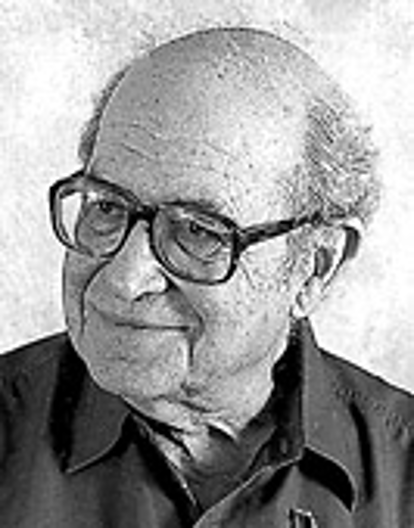
\includegraphics[width=\linewidth,height=0.5\textheight,keepaspectratio]{./images/cohen.png}

}

\caption{\label{fig-cohen}Dr.~Jacob Cohen (1923-1998)}

\end{figure}%
\end{column}
\end{columns}
\end{frame}

\begin{frame}{What Power Looks Like}
\phantomsection\label{what-power-looks-like}
\begin{center}
\pandocbounded{\includegraphics[keepaspectratio]{statistical-power-combined-t_files/figure-beamer/power-picture-1.png}}
\end{center}

\vspace{-0.2em}

\begin{center}
\footnotesize \textcolor{errorred}{\textbf{Red}} is the distribution of the test statistic if there is no effect; the shaded area past 1.96 is $\alpha$, the false-positive rate. \textcolor{statsecondary}{\textbf{Blue}} is the distribution if the effect is real; \textbf{the shaded area past the same line is power}.
\end{center}
\end{frame}

\begin{frame}{Core Notation}
\phantomsection\label{core-notation}
Power depends on four quantities:

\vspace{0.5em}

\begin{center}
\small
\setlength{\tabcolsep}{7pt}
\renewcommand{\arraystretch}{1.35}
\begin{tabular}{c>{\raggedright\arraybackslash}p{2.7cm}>{\raggedright\arraybackslash}p{5.6cm}>{\raggedright\arraybackslash}p{3.6cm}}
\toprule
\textbf{Symbol} & \textbf{Quantity} & \textbf{What it is} & \textbf{Can you change it?} \\
\midrule
$N$              & Sample size        & Total number of subjects. & Yes, within your budget. \\
$\mu_t - \mu_c$  & Effect size        & The true difference between treatment and control means. & Partly: dose, duration, framing. \\
$\sigma$         & Standard deviation & How much outcomes vary between subjects. & Partly: better measures, covariates. \\
$\alpha$         & Significance level & The false-positive rate you accept. & Yes; usually 0.05. \\
\bottomrule
\end{tabular}
\end{center}

\vspace{0.4em}

\begin{center}
\small Larger effects, smaller $\sigma$, and larger $N$ all raise power. In code and in the appendix we write the effect as $\delta$.
\end{center}
\end{frame}

\begin{frame}{The Formula for a Two-Arm Experiment}
\phantomsection\label{the-formula-for-a-two-arm-experiment}
\vspace{0.2em}

\begin{center}
$\displaystyle \text{power} \;=\; \Phi\!\left( \frac{|\mu_t - \mu_c|\sqrt{N}}{2\sigma} \;-\; \Phi^{-1}\!\left(1-\frac{\alpha}{2}\right) \right)$
\end{center}

\vspace{0.6em}

\small

\(\Phi\) is the standard normal CDF: \(\Phi(x)\) is the probability that
a standard normal variable is at or below \(x\). \(\Phi^{-1}\) is its
inverse: it returns the \(z\) value with a given area to its left.

\vspace{0.6em}

The formula holds when:

\begin{itemize}
\tightlist
\item
  subjects are randomly assigned to two arms of \(N/2\) each,
\item
  the outcome is normally distributed with the same \(\sigma\) in both
  arms,
\item
  the analysis is a two-sided difference-in-means test.
\end{itemize}

\vspace{0.4em}

\scriptsize Source: Coppock,
\textit{10 Things to Know About Statistical Power} (EGAP). EGAP writes
power as \(\beta\); we use \(\beta\) for the Type II error rate, so
power \(= 1-\beta\).
\end{frame}

\begin{frame}{A Running Example: Does the Message Move Opinion?}
\phantomsection\label{a-running-example-does-the-message-move-opinion}
\begin{notebox}
\small You are fielding a survey experiment with \textbf{164 respondents}, randomly assigned 50/50 to read a short informational message (treatment) or no message (control). Support for the policy is measured on a 0--100 feeling thermometer, and a pilot study supplies your assumptions.
\end{notebox}

\vspace{0.2em}

\begin{center}
\small
\setlength{\tabcolsep}{7pt}
\renewcommand{\arraystretch}{1.2}
\begin{tabular}{cc>{\raggedright\arraybackslash}p{7.4cm}}
\toprule
\textbf{Symbol} & \textbf{Value} & \textbf{Where it comes from} \\
\midrule
$N$      & 164  & Total respondents (82 per arm). \\
$\mu_t$  & 57   & Assumed mean support under treatment. \\
$\mu_c$  & 50   & Control mean, from the pilot. \\
$\sigma$ & 20   & Standard deviation, from the pilot. \\
$\alpha$ & 0.05 & Two-sided, by convention. \\
\bottomrule
\end{tabular}
\end{center}

\vspace{0.2em}

\small Assumed effect: \(\mu_t - \mu_c = 7\) points, or \(0.35\sigma\).
\textbf{What is the power to detect a 7-point effect with 164 respondents?}
\end{frame}

\begin{frame}{Step 1: Do the Arithmetic}
\phantomsection\label{step-1-do-the-arithmetic}
\vspace{0.2em}

\begin{align*}
\text{power} &= \Phi\!\left( \frac{|\mu_t - \mu_c|\sqrt{N}}{2\sigma} \;-\; \Phi^{-1}\!\left(1-\frac{\alpha}{2}\right) \right)
   && \text{\small the formula} \\[0.25em]
&= \Phi\!\left( \frac{7\,\sqrt{164}}{2(20)} \;-\; \textcolor{statsecondary}{1.96} \right)
   && \text{\small plug in; \;\; $\Phi^{-1}(0.975) = 1.96$} \\[0.25em]
&= \Phi\!\left( \textcolor{statsecondary}{\mathbf{2.24}} \;-\; 1.96 \right) \;=\; \textcolor{statsecondary}{\Phi(\mathbf{0.28})}
   && \text{\small $7 \times 12.81 / 40 = 2.24$}
\end{align*}

\vspace{0.5em}

\begin{center}
\small
$\underbrace{\mathbf{2.24}}_{\text{expected } z}$ \qquad
$\underbrace{\mathbf{1.96}}_{\text{critical value}}$ \qquad
$\underbrace{\mathbf{0.28}}_{\text{difference}}$
\end{center}

\vspace{0.5em}

\begin{center}
\scriptsize The smaller the difference between the expected $z$ and the critical value, the lower the power. \\
(The appendix shows how to find $1.96$ in the $z$-table.)
\end{center}
\end{frame}

\begin{frame}{Step 2: Read the Answer Off the Table}
\phantomsection\label{step-2-read-the-answer-off-the-table}
\begin{columns}[T]

\begin{column}{0.30\textwidth}
\vspace{0.6em}

\begin{center}
$\text{power} = \Phi(\mathbf{0.28})$
\end{center}

\vspace{0.5em}

\footnotesize
Split the $z$-score across the two margins of the table:

\vspace{0.4em}

\hspace{0.5em}$\mathbf{0.2}\;$ selects the \textbf{row}

\vspace{0.2em}

\hspace{0.5em}$\mathbf{0.08}$ selects the \textbf{column}

\vspace{0.5em}

The cell where they meet is the area to the \textit{left} of $z$, which is the power.
\end{column}

\begin{column}{0.70\textwidth}
\begin{center}
\scriptsize
\setlength{\tabcolsep}{2.4pt}
\renewcommand{\arraystretch}{1.25}
\begin{tabular}{c|cccccccccc}
\toprule
$z$ & .00 & .01 & .02 & .03 & .04 & .05 & .06 & .07 & \cellcolor{stataccbg}\textbf{.08} & .09 \\
\midrule
0.0 & .5000 & .5040 & .5080 & .5120 & .5160 & .5199 & .5239 & .5279 & \cellcolor{stataccbg}.5319 & .5359 \\
0.1 & .5398 & .5438 & .5478 & .5517 & .5557 & .5596 & .5636 & .5675 & \cellcolor{stataccbg}.5714 & .5753 \\
\cellcolor{stataccbg}\textbf{0.2} & \cellcolor{stataccbg}.5793 & \cellcolor{stataccbg}.5832 & \cellcolor{stataccbg}.5871 & \cellcolor{stataccbg}.5910 & \cellcolor{stataccbg}.5948 & \cellcolor{stataccbg}.5987 & \cellcolor{stataccbg}.6026 & \cellcolor{stataccbg}.6064 & \cellcolor{statorange}\textbf{\color{white}.6103} & \cellcolor{stataccbg}.6141 \\
0.3 & .6179 & .6217 & .6255 & .6293 & .6331 & .6368 & .6406 & .6443 & \cellcolor{stataccbg}.6480 & .6517 \\
0.4 & .6554 & .6591 & .6628 & .6664 & .6700 & .6736 & .6772 & .6808 & \cellcolor{stataccbg}.6844 & .6879 \\
0.5 & .6915 & .6950 & .6985 & .7019 & .7054 & .7088 & .7123 & .7157 & \cellcolor{stataccbg}.7190 & .7224 \\
\bottomrule
\end{tabular}
\end{center}
\end{column}

\end{columns}

\vspace{0.5em}

\begin{center}
\large $\text{power} \;=\; \Phi(0.28) \;=\; \textcolor{statorange}{\mathbf{0.61}}$
\end{center}
\end{frame}

\begin{frame}{The Smallest Effect This Study Can Detect}
\phantomsection\label{the-smallest-effect-this-study-can-detect}
\small Fix power at 80\% and solve the same formula for the effect. The
result is the \textbf{minimum detectable effect} (MDE).

\vspace{0.3em}

\begin{center}
$\displaystyle \text{MDE} \;=\; \underbrace{\left(\Phi^{-1}\!\left(1-\tfrac{\alpha}{2}\right) + \Phi^{-1}(0.80)\right)}_{1.96 \;+\; 0.84 \;=\; 2.80} \;\times\; \underbrace{\frac{2\sigma}{\sqrt{N}}}_{\text{standard error}}$
\end{center}

\vspace{0.3em}

\begin{center}
\scriptsize
\setlength{\tabcolsep}{9pt}
\renewcommand{\arraystretch}{1.08}
\begin{tabular}{ccc}
\toprule
$N$ & \textbf{Minimum detectable effect} & \textbf{In standard deviations} \\
\midrule
\textcolor{statorange}{\textbf{164}} & \textcolor{statorange}{\textbf{8.75 points}} & \textcolor{statorange}{\textbf{0.44$\sigma$}} \\
257  & 6.99 & 0.35$\sigma$ \\
400  & 5.60 & 0.28$\sigma$ \\
800  & 3.96 & 0.20$\sigma$ \\
1396 & 3.00 & 0.15$\sigma$ \\
\bottomrule
\end{tabular}
\end{center}

\vspace{0.2em}

\begin{center}
\small The pilot assumes 7 points, but with 164 respondents only effects of $\textcolor{statorange}{\mathbf{8.75}}$ points or more have 80\% power. \\[0.3em]
\footnotesize Solved for $N$ instead: \; $N = 4\sigma^2\big(z_{1-\alpha/2} + z_{0.80}\big)^2 / (\mu_t - \mu_c)^2$.
\end{center}
\end{frame}

\begin{frame}{Your Turn: Is the Tutoring Program Worth Studying?}
\phantomsection\label{your-turn-is-the-tutoring-program-worth-studying}
\vspace{0.5em}

\begin{notebox}
\small A colleague is evaluating a new tutoring program. \textbf{400 students} will be randomly assigned, 200 to tutoring and 200 to business as usual, with final exam score as the outcome. Past cohorts averaged \textbf{72} points with a standard deviation of \textbf{10}, and the program is expected to add \textbf{3} points.
\end{notebox}

\vspace{0.7em}

\begin{center}
\large \textbf{What is the power of this design?}
\end{center}

\vspace{0.7em}

\begin{columns}[c]

\begin{column}{0.46\textwidth}
\begin{center}
\footnotesize
\setlength{\tabcolsep}{10pt}
\renewcommand{\arraystretch}{1.2}
\begin{tabular}{cc}
\toprule
\textbf{Symbol} & \textbf{Value} \\
\midrule
$N$      & 400  \\
$\mu_t$  & 75   \\
$\mu_c$  & 72   \\
$\sigma$ & 10   \\
$\alpha$ & 0.05, two-sided \\
\bottomrule
\end{tabular}
\end{center}
\end{column}

\begin{column}{0.50\textwidth}
\footnotesize
The formula and the $z$-table are on your \textbf{handout}.

\vspace{0.6em}

Work it in three steps:

\vspace{0.3em}

\hspace{0.4em}1. Compute the expected $z$

\vspace{0.2em}

\hspace{0.4em}2. Subtract the critical value

\vspace{0.2em}

\hspace{0.4em}3. Look the difference up in the table

\vspace{0.6em}

\textit{If you finish early:} what is the MDE at $N = 400$?
\end{column}

\end{columns}
\end{frame}

\begin{frame}{Your Turn: The Solution}
\phantomsection\label{your-turn-the-solution}
\vspace{0.2em}

\begin{align*}
\text{power} &= \Phi\!\left( \frac{|75 - 72|\,\sqrt{400}}{2(10)} \;-\; \Phi^{-1}\!\left(1-\tfrac{0.05}{2}\right) \right)
   && \text{\small \textbf{Step 1:} plug in} \\[0.25em]
&= \Phi\!\left( \frac{3 \times 20}{20} \;-\; 1.96 \right)
   && \text{\small \textbf{Step 2:} $\sqrt{400} = 20$; $\Phi^{-1}(0.975) = 1.96$} \\[0.25em]
&= \Phi(3.00 - 1.96) \;=\; \textcolor{statsecondary}{\Phi(\mathbf{1.04})}
   && \text{\small \textbf{Step 3:} simplify} \\[0.25em]
&= \mathbf{0.85}
   && \text{\small \textbf{Step 4:} row $1.0$, column $.04 \to .8508$}
\end{align*}

\vspace{0.4em}

\begin{center}
\small MDE at $N = 400$: \; $2.80 \times 2(10)/\sqrt{400} = \mathbf{2.80}$ points.
\end{center}
\end{frame}

\begin{frame}{Check Your Work: The EGAP Power Calculator}
\phantomsection\label{check-your-work-the-egap-power-calculator}
\vspace{0.3em}

\begin{center}
\small \url{https://egap.shinyapps.io/power-app/}
\end{center}

\vspace{0.6em}

\begin{center}
\small
\setlength{\tabcolsep}{7pt}
\renewcommand{\arraystretch}{1.25}
\begin{tabular}{c>{\raggedright\arraybackslash}p{6.4cm}c}
\toprule
\textbf{Our symbol} & \textbf{Field in the app} & \textbf{Enter} \\
\midrule
$\mu_t - \mu_c$ & Treatment Effect Size                  & 3    \\
$\sigma$        & Standard Deviation of Outcome Variable & 10   \\
$\alpha$        & Significance Level                     & 0.05 \\
                & Power Target                           & 0.8  \\
                & Maximum Number of Subjects             & 800  \\
\bottomrule
\end{tabular}
\end{center}

\vspace{0.5em}

\begin{center}
\small Leave \textit{Clustered Design} and \textit{Binary Dependent Variable} unchecked. (The appendix shows what clustering does to $N$.)
\end{center}
\end{frame}

\begin{frame}{Reading the Power Curve}
\phantomsection\label{reading-the-power-curve}
\begin{columns}[c]

\begin{column}{0.53\textwidth}
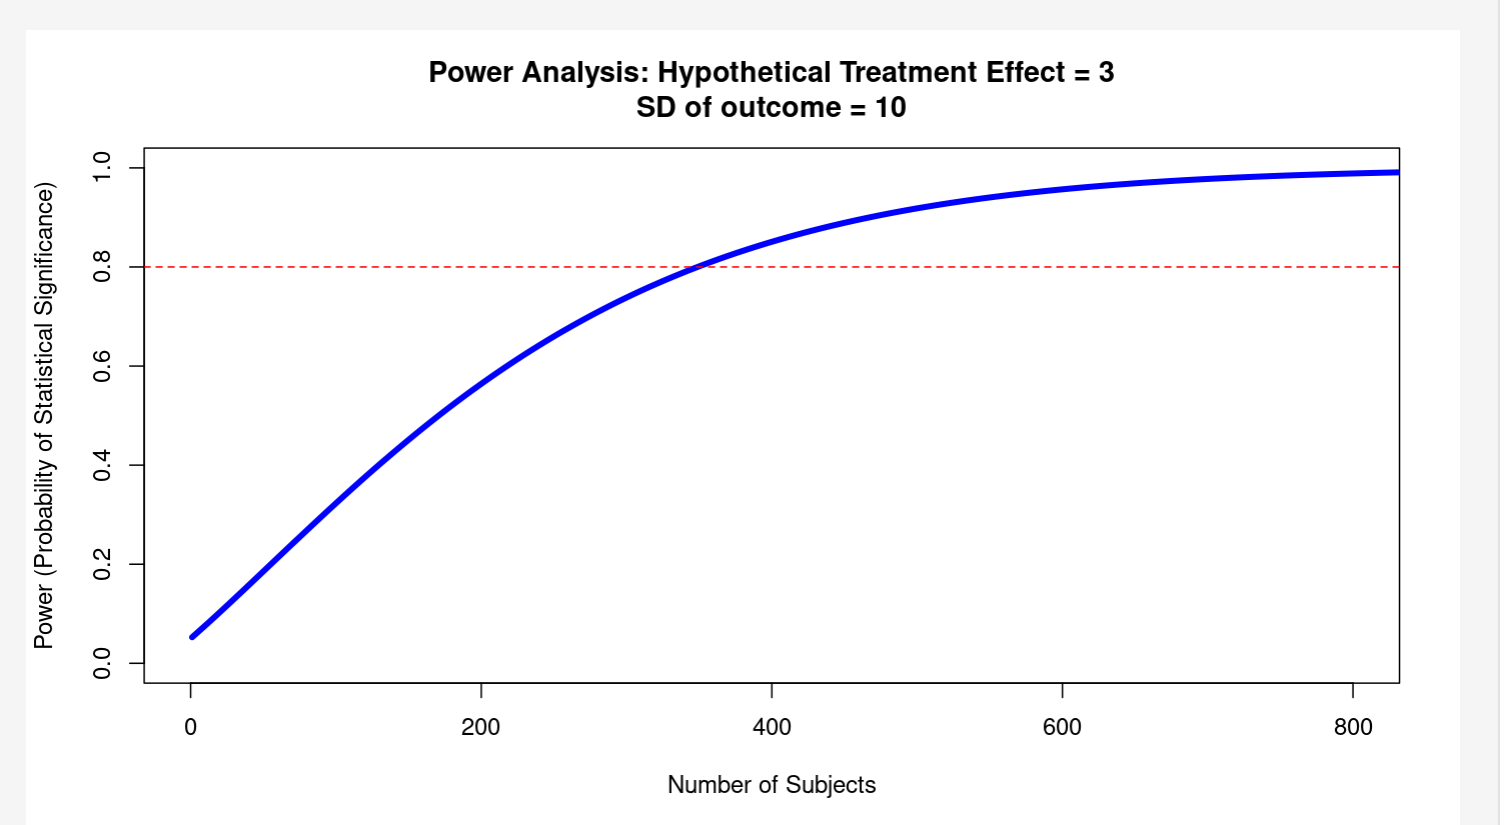
\includegraphics[width=\linewidth]{images/egap-power-app.png}
\end{column}

\begin{column}{0.45\textwidth}
\footnotesize
\setlength{\itemsep}{0.35em}
\begin{itemize}
\item The $x$-axis is \textbf{total sample size}; the $y$-axis is \textbf{power}.
\item The blue curve shows power as $N$ grows, holding the effect at 3 and $\sigma$ at 10.
\item The red dashed line marks the \textbf{80\% target}. The curve crosses it at the $N$ you need: \textbf{349}.
\item Our $N = 400$ is to the \textit{right} of that point. Reading up from 400 gives $\approx \mathbf{0.85}$.
\item The curve flattens: past about 600 students, each additional student adds little power.
\end{itemize}
\end{column}

\end{columns}
\end{frame}

\begin{frame}{Where Do the Assumptions Come From?}
\phantomsection\label{where-do-the-assumptions-come-from}
\small Power calculations are most useful \textit{before} data
collection, so every input is an estimate. \textbf{In pairs:} pick a
study one of you is planning. For each row, say where your number would
come from.

\begin{center}
\footnotesize
\setlength{\tabcolsep}{7pt}
\renewcommand{\arraystretch}{1.0}
\begin{tabular}{>{\raggedright\arraybackslash}p{4.0cm}>{\raggedright\arraybackslash}p{8.7cm}}
\toprule
\textbf{The estimate} & \textbf{Possible sources} \\
\midrule
How big an effect should I expect? \newline \textcolor{statsecondary}{$\mu_t - \mu_c$, \; $\sigma$}
& \leavevmode\uncover<2->{\textbullet~Published effects, discounted for publication bias}\newline
\uncover<2->{\textbullet~A pilot or baseline wave, which gives $\sigma$ directly}\newline
\uncover<2->{\textbullet~The \textit{smallest} effect that would change a decision} \\
\midrule
How many people can I afford to treat? \newline \textcolor{statsecondary}{$N$}
& \leavevmode\uncover<3->{\textbullet~Budget divided by cost per subject}\newline
\uncover<3->{\textbullet~Field period, staff time, partner capacity}\newline
\uncover<3->{\textbullet~Size of the population you can reach} \\
\midrule
How many will respond and stay? \newline \textcolor{statsecondary}{$N$ analyzed}
& \leavevmode\uncover<4->{\textbullet~Response rates from earlier waves or similar surveys}\newline
\uncover<4->{\textbullet~Attrition rates in similar designs}\newline
\uncover<4->{\textbullet~Compute power for the $N$ you will analyze, not the $N$ you invite} \\
\bottomrule
\end{tabular}
\end{center}

\vspace{-0.6em}

\uncover<5->{\begin{center}
\footnotesize Each source gives a range, not a single number. The next step is to compute power across that range.
\end{center}}
\end{frame}

\begin{frame}{What If We Don't Know the Effect?}
\phantomsection\label{what-if-we-dont-know-the-effect}
\vspace{0.2em}

\small Back to the survey experiment. The pilot fixed everything
\textit{except} the expected effect size.

\vspace{0.5em}

\begin{columns}[T]

\begin{column}{0.40\textwidth}
\begin{center}
\footnotesize
\setlength{\tabcolsep}{6pt}
\renewcommand{\arraystretch}{1.25}
\begin{tabular}{cc}
\toprule
\multicolumn{2}{c}{\textbf{Fixed by the pilot}} \\
\midrule
$\mu_c$        & 50   \\
$\sigma$       & 20   \\
$\alpha$       & 0.05 \\
target power & 0.80 \\
\midrule
$\mu_t - \mu_c$ & \textcolor{statorange}{\textbf{?}} \\
$N$             & \textcolor{statorange}{\textbf{?}} \\
\bottomrule
\end{tabular}
\end{center}
\end{column}

\begin{column}{0.58\textwidth}
\begin{center}
\footnotesize
\setlength{\tabcolsep}{6pt}
\renewcommand{\arraystretch}{1.25}
\begin{tabular}{>{\raggedright\arraybackslash}p{5.6cm}c}
\toprule
\textbf{Source of the effect} & $\mu_t - \mu_c$ \\
\midrule
Our own pilot                          & 7 \\
A published study of a similar message & 5 \\
That published effect, discounted for publication bias & 3 \\
\bottomrule
\end{tabular}
\end{center}
\end{column}

\end{columns}

\vspace{0.6em}

\begin{center}
\small Instead of choosing one, compute power for all three across a range of $N$.
\end{center}
\end{frame}

\begin{frame}[fragile]{The Formula, in Code}
\phantomsection\label{the-formula-in-code}
\vspace{0.6em}

\begin{center}
$\displaystyle \text{power} \;=\; \Phi\!\left( \frac{|\mu_t - \mu_c|\sqrt{N}}{2\sigma} \;-\; \Phi^{-1}\!\left(1-\frac{\alpha}{2}\right) \right)$
\end{center}

\vspace{0.9em}

\begin{Shaded}
\begin{Highlighting}[]
\NormalTok{power\_calc }\OtherTok{\textless{}{-}} \ControlFlowTok{function}\NormalTok{(mu\_t, mu\_c, sigma, N, }\AttributeTok{alpha =} \FloatTok{0.05}\NormalTok{) \{}
\NormalTok{  z }\OtherTok{\textless{}{-}} \FunctionTok{abs}\NormalTok{(mu\_t }\SpecialCharTok{{-}}\NormalTok{ mu\_c) }\SpecialCharTok{*} \FunctionTok{sqrt}\NormalTok{(N) }\SpecialCharTok{/}\NormalTok{ (}\DecValTok{2} \SpecialCharTok{*}\NormalTok{ sigma)}
\NormalTok{  cv }\OtherTok{\textless{}{-}} \FunctionTok{qnorm}\NormalTok{(}\DecValTok{1} \SpecialCharTok{{-}}\NormalTok{ alpha }\SpecialCharTok{/} \DecValTok{2}\NormalTok{)}
  \FunctionTok{pnorm}\NormalTok{(z }\SpecialCharTok{{-}}\NormalTok{ cv) }\SpecialCharTok{+} \FunctionTok{pnorm}\NormalTok{(}\SpecialCharTok{{-}}\NormalTok{z }\SpecialCharTok{{-}}\NormalTok{ cv) }\CommentTok{\# both rejection tails}
\NormalTok{\}}
\end{Highlighting}
\end{Shaded}

\vspace{0.9em}

\begin{center}
\large $\Phi \;=\;$ \texttt{pnorm} \qquad\qquad $\Phi^{-1} \;=\;$ \texttt{qnorm}
\end{center}
\end{frame}

\begin{frame}[fragile]{Power Across a Range of \(N\)}
\phantomsection\label{power-across-a-range-of-n}
\begin{Shaded}
\begin{Highlighting}[]
\NormalTok{grid }\OtherTok{\textless{}{-}} \FunctionTok{expand.grid}\NormalTok{(}\AttributeTok{N =} \FunctionTok{seq}\NormalTok{(}\DecValTok{60}\NormalTok{, }\DecValTok{1600}\NormalTok{, }\AttributeTok{by =} \DecValTok{10}\NormalTok{), }\AttributeTok{delta =} \FunctionTok{c}\NormalTok{(}\DecValTok{3}\NormalTok{, }\DecValTok{5}\NormalTok{, }\DecValTok{7}\NormalTok{))}

\NormalTok{grid}\SpecialCharTok{$}\NormalTok{power }\OtherTok{\textless{}{-}} \FunctionTok{power\_calc}\NormalTok{(}
  \AttributeTok{mu\_t =} \DecValTok{50} \SpecialCharTok{+}\NormalTok{ grid}\SpecialCharTok{$}\NormalTok{delta,}
  \AttributeTok{mu\_c =} \DecValTok{50}\NormalTok{,}
  \AttributeTok{sigma =} \DecValTok{20}\NormalTok{,}
  \AttributeTok{N =}\NormalTok{ grid}\SpecialCharTok{$}\NormalTok{N}
\NormalTok{)}

\FunctionTok{head}\NormalTok{(grid, }\DecValTok{3}\NormalTok{)}
\end{Highlighting}
\end{Shaded}

\begin{verbatim}
   N delta      power
1 60     3 0.08947303
2 70     3 0.09618740
3 80     3 0.10293349
\end{verbatim}

\vspace{0.4em}

\begin{center}
\small Three effect sizes $\times$ 155 values of $N$ = 465 rows. Next, plot \texttt{power} against \texttt{N}.
\end{center}
\end{frame}

\begin{frame}{How Many Respondents Do We Need?}
\phantomsection\label{how-many-respondents-do-we-need}
\begin{center}
\pandocbounded{\includegraphics[keepaspectratio]{statistical-power-combined-t_files/figure-beamer/sweep-plot-1.png}}
\end{center}
\end{frame}

\begin{frame}{Your Turn (Groups): A Sleep Workshop on a Budget}
\phantomsection\label{your-turn-groups-a-sleep-workshop-on-a-budget}
\small The campus wellness office wants to test a two-session
\textbf{sleep workshop} for undergraduates. Students are randomized to
the workshop or a waitlist and wear a sleep tracker for two weeks
afterward. The outcome is average nightly sleep, in minutes.

\vspace{0.4em}

\begin{columns}[T]
\begin{column}{0.4\linewidth}
\begin{center}
\footnotesize
\setlength{\tabcolsep}{6pt}
\renewcommand{\arraystretch}{1.2}
\begin{tabular}{cc}
\toprule
\multicolumn{2}{c}{\textbf{From last year's tracker data}} \\
\midrule
$\mu_c$  & 400 minutes \\
$\sigma$ & 60 minutes \\
$\alpha$ & 0.05 \\
\midrule
\multicolumn{2}{c}{\textbf{Budget}} \\
\midrule
Cost per student & \$40 \\
Total            & \$12{,}000 \\
\bottomrule
\end{tabular}
\end{center}
\end{column}

\begin{column}{0.58\linewidth}
\footnotesize
\textbf{Three sources disagree about the effect:}

\vspace{0.3em}

\begin{tabular}{>{\raggedright\arraybackslash}p{5.6cm}r}
\toprule
\textbf{Source} & \textbf{Effect} \\
\midrule
A pilot with 20 students & +25 min \\
A meta-analysis of similar brief workshops & +15 min \\
The office director: ``Under 10 minutes isn't worth running the workshop'' & +10 min \\
\bottomrule
\end{tabular}

\vspace{0.4em}

\textit{All numbers are hypothetical.}
\end{column}
\end{columns}
\end{frame}

\begin{frame}[fragile]{Your Turn (Groups): What to Produce}
\phantomsection\label{your-turn-groups-what-to-produce}
\small Work in groups of 3--4. You have about 12 minutes. Open
\texttt{scripts/sleep\_group\_activity.R}.

\vspace{0.3em}

\footnotesize
\begin{enumerate}
\item \textbf{Discuss:} which source would you trust most, and what is wrong with each one?
\item \textbf{Sweep:} choose the effect sizes to plan for, and find the smallest $N$ that reaches 80\% power for each.
\item \textbf{Budget:} how many students does \$12{,}000 pay for? Which of your effects can that $N$ detect?
\item \textbf{Report:} write the sentence your group would put in a proposal: \textit{``With N = \_\_\_, the study has 80\% power to detect effects of \_\_\_ minutes or larger.''}
\end{enumerate}

\begin{Shaded}
\begin{Highlighting}[]
\NormalTok{grid }\OtherTok{\textless{}{-}} \FunctionTok{expand.grid}\NormalTok{(}\AttributeTok{N =} \FunctionTok{seq}\NormalTok{(\_\_\_, \_\_\_, }\AttributeTok{by =} \DecValTok{10}\NormalTok{),}
                    \AttributeTok{delta =} \FunctionTok{c}\NormalTok{(\_\_\_, \_\_\_, \_\_\_))}
\NormalTok{grid}\SpecialCharTok{$}\NormalTok{power }\OtherTok{\textless{}{-}} \FunctionTok{power\_calc}\NormalTok{(}\AttributeTok{mu\_t =}\NormalTok{ mu\_c }\SpecialCharTok{+}\NormalTok{ grid}\SpecialCharTok{$}\NormalTok{delta, }\AttributeTok{mu\_c =}\NormalTok{ mu\_c,}
                         \AttributeTok{sigma =}\NormalTok{ sigma, }\AttributeTok{N =}\NormalTok{ grid}\SpecialCharTok{$}\NormalTok{N)}
\end{Highlighting}
\end{Shaded}
\end{frame}

\begin{frame}[fragile]{Your Turn (Groups): One Solution}
\phantomsection\label{your-turn-groups-one-solution}
\begin{Shaded}
\begin{Highlighting}[]
\NormalTok{grid }\OtherTok{\textless{}{-}} \FunctionTok{expand.grid}\NormalTok{(}\AttributeTok{N =} \FunctionTok{seq}\NormalTok{(}\DecValTok{50}\NormalTok{, }\DecValTok{1500}\NormalTok{, }\AttributeTok{by =} \DecValTok{10}\NormalTok{), }\AttributeTok{delta =} \FunctionTok{c}\NormalTok{(}\DecValTok{10}\NormalTok{, }\DecValTok{15}\NormalTok{, }\DecValTok{25}\NormalTok{))}
\NormalTok{grid}\SpecialCharTok{$}\NormalTok{power }\OtherTok{\textless{}{-}} \FunctionTok{power\_calc}\NormalTok{(}\DecValTok{400} \SpecialCharTok{+}\NormalTok{ grid}\SpecialCharTok{$}\NormalTok{delta, }\DecValTok{400}\NormalTok{, }\AttributeTok{sigma =} \DecValTok{60}\NormalTok{, }\AttributeTok{N =}\NormalTok{ grid}\SpecialCharTok{$}\NormalTok{N)}

\CommentTok{\# smallest N with 80\% power, for effects of 10, 15, and 25 minutes}
\FunctionTok{sapply}\NormalTok{(}\FunctionTok{c}\NormalTok{(}\DecValTok{10}\NormalTok{, }\DecValTok{15}\NormalTok{, }\DecValTok{25}\NormalTok{), \textbackslash{}(d) }\FunctionTok{min}\NormalTok{(grid}\SpecialCharTok{$}\NormalTok{N[grid}\SpecialCharTok{$}\NormalTok{delta }\SpecialCharTok{==}\NormalTok{ d }\SpecialCharTok{\&}\NormalTok{ grid}\SpecialCharTok{$}\NormalTok{power }\SpecialCharTok{\textgreater{}=} \FloatTok{0.8}\NormalTok{]))}
\end{Highlighting}
\end{Shaded}

\begin{verbatim}
[1] 1140  510  190
\end{verbatim}

\begin{Shaded}
\begin{Highlighting}[]
\NormalTok{mde\_300 }\OtherTok{\textless{}{-}}\NormalTok{ (}\FunctionTok{qnorm}\NormalTok{(}\FloatTok{0.975}\NormalTok{) }\SpecialCharTok{+} \FunctionTok{qnorm}\NormalTok{(}\FloatTok{0.80}\NormalTok{)) }\SpecialCharTok{*} \DecValTok{2} \SpecialCharTok{*} \DecValTok{60} \SpecialCharTok{/} \FunctionTok{sqrt}\NormalTok{(}\DecValTok{300}\NormalTok{) }\CommentTok{\# $12,000 / $40}
\FunctionTok{round}\NormalTok{(mde\_300, }\DecValTok{1}\NormalTok{)}
\end{Highlighting}
\end{Shaded}

\begin{verbatim}
[1] 19.4
\end{verbatim}

\footnotesize The budget pays for 300 students, enough to detect effects
of 19.4 minutes or more. That covers the pilot's 25 minutes, but a pilot
of 20 students gives a noisy estimate. The meta-analysis's 15 minutes
needs about 510 students (\$20,400).
\end{frame}

\begin{frame}{Break}
\phantomsection\label{break}
\vspace{3em}

\begin{center}
\Large 5 minutes
\end{center}
\end{frame}

\begin{frame}{Where the Formula Stops Applying}
\phantomsection\label{where-the-formula-stops-applying}
\small The formula covers one design: two arms, a normal outcome, a
difference in means. Other tests have their own formulas, and many
designs have none.

\vspace{0.4em}

\begin{center}
\small
\setlength{\tabcolsep}{7pt}
\renewcommand{\arraystretch}{1.2}
\begin{tabular}{>{\raggedright\arraybackslash}p{5.3cm}>{\raggedright\arraybackslash}p{7.4cm}}
\toprule
\textbf{The formula assumes} & \textbf{So it does not cover} \\
\midrule
Two arms, split 50/50            & Three arms, unequal allocation \\
One continuous, normal outcome   & Binary outcomes, counts, skewed scales \\
A simple difference in means     & Covariates, fixed effects, IV, mixed models \\
Independent observations         & Clustered or repeated measures \\
Everyone recruited is analyzed   & Attrition, non-response \\
A significance test              & Bayesian or estimation-based goals \\
\bottomrule
\end{tabular}
\end{center}
\end{frame}

\begin{frame}{A More General Definition of Power}
\phantomsection\label{a-more-general-definition-of-power}
\vspace{1em}

\begin{center}
\large Power is the probability that the analysis \textcolor{statsecondary}{\textbf{recovers}} a real effect, if one exists.
\end{center}

\vspace{1.5em}

\small

\begin{itemize}
\tightlist
\item
  So far, ``recovers'' has meant \(p < 0.05\).
\item
  In a simulation, it can mean any criterion you can check in code: the
  estimate is within a set distance of the truth, the confidence
  interval excludes zero, a posterior probability exceeds 0.95.
\item
  With this definition, power can be estimated for any design whose data
  you can simulate.
\end{itemize}
\end{frame}

\begin{frame}{Monte Carlo Simulation}
\phantomsection\label{monte-carlo-simulation}
\begin{columns}[T]
\begin{column}{0.62\linewidth}
\small

\begin{itemize}
\tightlist
\item
  Monte Carlo methods estimate a quantity by repeated random sampling.
\item
  They are useful when there is no closed-form answer, which is the case
  for most study designs.
\item
  The quantity being estimated is fixed; the random sampling is only the
  method for computing it.
\item
  Any quantity that can be written as a probability can be estimated
  this way.
\end{itemize}
\end{column}

\begin{column}{0.38\linewidth}
\begin{figure}

\centering{

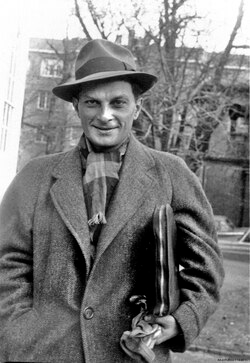
\includegraphics[width=\linewidth,height=0.5\textheight,keepaspectratio]{./images/ulam.png}

}

\caption{\label{fig-ulam}Stanisław Ulam developed the method in the
1940s. It is named after the casino in Monaco, where his uncle gambled.}

\end{figure}%
\end{column}
\end{columns}
\end{frame}

\begin{frame}{Monte Carlo Simulation: A Roulette Example}
\phantomsection\label{monte-carlo-simulation-a-roulette-example}
\begin{columns}[T]
\begin{column}{0.58\linewidth}
\small

Start with a gambling problem that has an exact answer:

\vspace{0.5em}

\begin{center}
What is the probability of winning on red three spins in a row?
\end{center}

\vspace{0.5em}

\begin{itemize}
\tightlist
\item
  A roulette wheel has 38 pockets, 18 of them red.
\item
  Each spin is independent, so
\end{itemize}

\[
P(\text{3 reds in a row}) = (18/38)^3 \approx 0.106
\]

\begin{itemize}
\tightlist
\item
  Next: estimate the same number by simulating spins, and compare.
\end{itemize}
\end{column}

\begin{column}{0.42\linewidth}
\begin{figure}

\centering{

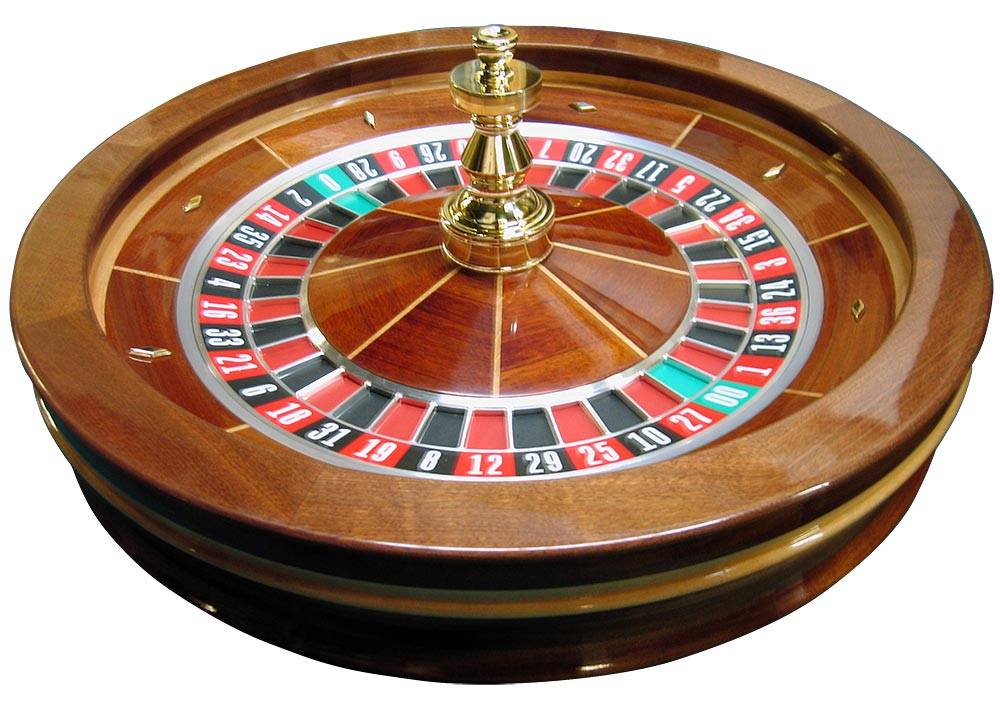
\includegraphics[width=\linewidth,height=0.5\textheight,keepaspectratio]{./images/roulette.png}

}

\caption{\label{fig-roulette}A standard roulette table}

\end{figure}%
\end{column}
\end{columns}
\end{frame}

\begin{frame}[fragile]{Monte Carlo Simulation: Simulating the Spins}
\phantomsection\label{monte-carlo-simulation-simulating-the-spins}
Simulate 100,000 sets of three spins and count how often all three are
red:

\begin{Shaded}
\begin{Highlighting}[]
\FunctionTok{set.seed}\NormalTok{(}\DecValTok{2026}\NormalTok{)}
\NormalTok{spins }\OtherTok{\textless{}{-}} \FunctionTok{matrix}\NormalTok{(}\FunctionTok{runif}\NormalTok{(}\DecValTok{3} \SpecialCharTok{*} \DecValTok{100000}\NormalTok{) }\SpecialCharTok{\textless{}} \DecValTok{18} \SpecialCharTok{/} \DecValTok{38}\NormalTok{, }\AttributeTok{ncol =} \DecValTok{3}\NormalTok{) }\CommentTok{\# each row is 3 spins}
\FunctionTok{mean}\NormalTok{(}\FunctionTok{rowSums}\NormalTok{(spins) }\SpecialCharTok{==} \DecValTok{3}\NormalTok{) }\CommentTok{\# proportion of rows where all three are red}
\end{Highlighting}
\end{Shaded}

\begin{verbatim}
[1] 0.1059
\end{verbatim}

\vspace{0.6em}

\begin{center}
\small If you can write down how the data are generated, you can estimate a probability by running that process many times and counting. Power is a probability, so it can be estimated the same way.
\end{center}
\end{frame}

\begin{frame}[fragile]{The Simulation Recipe}
\phantomsection\label{the-simulation-recipe}
\small Write three functions:

\begin{itemize}
\tightlist
\item
  \texttt{generate()}: make one fake data set from the model you expect
  your data to follow
\item
  \texttt{analyze()}: run the analysis you will run on the real data
\item
  \texttt{success()}: return \texttt{TRUE} if this run recovered the
  effect
\end{itemize}

Then run them many times. The proportion of successes is the estimated
power:

\begin{Shaded}
\begin{Highlighting}[]
\NormalTok{simulate\_power }\OtherTok{\textless{}{-}} \ControlFlowTok{function}\NormalTok{(n\_sims, generate, analyze, success) \{}
\NormalTok{  hits }\OtherTok{\textless{}{-}} \FunctionTok{replicate}\NormalTok{(n\_sims, }\FunctionTok{success}\NormalTok{(}\FunctionTok{analyze}\NormalTok{(}\FunctionTok{generate}\NormalTok{())))}
  \FunctionTok{mean}\NormalTok{(hits) }\CommentTok{\# proportion of successful runs = power}
\NormalTok{\}}
\end{Highlighting}
\end{Shaded}
\end{frame}

\begin{frame}[fragile]{Generating Data for the Tutoring Study}
\phantomsection\label{generating-data-for-the-tutoring-study}
For student \(i\):

\[
\text{post}_i = \underbrace{\mu_c}_{\text{control mean}} + \underbrace{\delta \, T_i}_{\text{tutoring effect}} + \underbrace{\varepsilon_i}_{\text{noise}}, \qquad \varepsilon_i \sim N(0, \sigma^2)
\]

\footnotesize \(\mu_c = 72\); ; \(T_i = 1\) if student \(i\) was
tutored, 0 if not; ; \(\delta = 3\); ; \(\sigma = 10\). We use
\(N = 350\), close to the 349 the EGAP curve gave for 80\% power.

\begin{Shaded}
\begin{Highlighting}[]
\NormalTok{gen\_basic }\OtherTok{\textless{}{-}} \ControlFlowTok{function}\NormalTok{(}\AttributeTok{n =} \DecValTok{350}\NormalTok{, }\AttributeTok{effect =} \DecValTok{3}\NormalTok{, }\AttributeTok{sd =} \DecValTok{10}\NormalTok{) \{}
\NormalTok{  treat }\OtherTok{\textless{}{-}} \FunctionTok{rep}\NormalTok{(}\DecValTok{0}\SpecialCharTok{:}\DecValTok{1}\NormalTok{, }\AttributeTok{each =}\NormalTok{ n }\SpecialCharTok{/} \DecValTok{2}\NormalTok{) }\CommentTok{\# half control, half tutored}
\NormalTok{  post }\OtherTok{\textless{}{-}} \DecValTok{72} \SpecialCharTok{+}\NormalTok{ effect }\SpecialCharTok{*}\NormalTok{ treat }\SpecialCharTok{+} \FunctionTok{rnorm}\NormalTok{(n, }\AttributeTok{mean =} \DecValTok{0}\NormalTok{, }\AttributeTok{sd =}\NormalTok{ sd)}
  \FunctionTok{data.frame}\NormalTok{(treat, post)}
\NormalTok{\}}
\end{Highlighting}
\end{Shaded}
\end{frame}

\begin{frame}[fragile]{Analyzing It and Defining Success}
\phantomsection\label{analyzing-it-and-defining-success}
\begin{Shaded}
\begin{Highlighting}[]
\NormalTok{analyze\_lm }\OtherTok{\textless{}{-}} \ControlFlowTok{function}\NormalTok{(dat) \{}
\NormalTok{  fit }\OtherTok{\textless{}{-}} \FunctionTok{lm}\NormalTok{(post }\SpecialCharTok{\textasciitilde{}}\NormalTok{ treat, }\AttributeTok{data =}\NormalTok{ dat) }\CommentTok{\# same as an equal{-}variance t{-}test}
  \FunctionTok{summary}\NormalTok{(fit)}\SpecialCharTok{$}\NormalTok{coefficients[}\StringTok{"treat"}\NormalTok{, ] }\CommentTok{\# estimate, SE, t, p for treat}
\NormalTok{\}}

\NormalTok{success\_sig }\OtherTok{\textless{}{-}} \ControlFlowTok{function}\NormalTok{(est) \{}
\NormalTok{  est[[}\StringTok{"Pr(\textgreater{}|t|)"}\NormalTok{]] }\SpecialCharTok{\textless{}} \FloatTok{0.05} \CommentTok{\# did we reject the null?}
\NormalTok{\}}

\FunctionTok{analyze\_lm}\NormalTok{(}\FunctionTok{gen\_basic}\NormalTok{())}
\end{Highlighting}
\end{Shaded}

\begin{verbatim}
  Estimate Std. Error    t value   Pr(>|t|) 
 3.0384590  1.1588225  2.6220228  0.0091249 
\end{verbatim}

\vspace{0.3em}

\begin{center}
\small \textbf{Predict:} the formula gives power = 0.8 at $N = 350$. What will 2,000 simulated studies give?
\end{center}
\end{frame}

\begin{frame}[fragile]{Does the Simulation Agree with the Formula?}
\phantomsection\label{does-the-simulation-agree-with-the-formula}
\begin{Shaded}
\begin{Highlighting}[]
\FunctionTok{set.seed}\NormalTok{(}\DecValTok{2026}\NormalTok{)}
\FunctionTok{simulate\_power}\NormalTok{(}\AttributeTok{n\_sims =} \DecValTok{2000}\NormalTok{, }\AttributeTok{generate =}\NormalTok{ gen\_basic,}
               \AttributeTok{analyze =}\NormalTok{ analyze\_lm, }\AttributeTok{success =}\NormalTok{ success\_sig)}
\end{Highlighting}
\end{Shaded}

\begin{verbatim}
[1] 0.8105
\end{verbatim}

\vspace{0.4em}

\small The formula gives 0.8. The simulated estimate has its own error.
With \(S\) simulations, the Monte Carlo standard error is

\[
\text{SE} = \sqrt{\frac{p(1-p)}{S}}
\]

which is about 0.009 for \(p = 0.80\) and \(S = 2{,}000\). For a more
precise estimate, increase \(S\).
\end{frame}

\begin{frame}{Adding a Pre-Test}
\phantomsection\label{adding-a-pre-test}
\small Schools often have each student's \textbf{pre-test score}. The
model for student \(i\) becomes:

\[
\text{pre}_i \sim N(70, \sigma^2)
\]

\[
\text{post}_i = \mu_c +
\underbrace{\rho\,(\text{pre}_i - 70)}_{\text{prior achievement}} +
\delta \, T_i +
\varepsilon_i,
\qquad \varepsilon_i \sim N\big(0,\ \sigma^2(1-\rho^2)\big)
\]

\begin{itemize}
\tightlist
\item
  \(\rho = 0.6\) is the correlation between pre-test and end-of-term
  scores.
\item
  The total standard deviation of post-test scores is still
  \(\sigma = 10\).
\end{itemize}

\vspace{0.4em}

\begin{center}
\textbf{Predict:} at the same $N = 350$, does adjusting for the pre-test raise or lower power? By how much?
\end{center}
\end{frame}

\begin{frame}[fragile]{Adjusting for the Pre-Test: Code}
\phantomsection\label{adjusting-for-the-pre-test-code}
\small Only \texttt{generate()} and \texttt{analyze()} change:

\begin{Shaded}
\begin{Highlighting}[]
\NormalTok{gen\_pretest }\OtherTok{\textless{}{-}} \ControlFlowTok{function}\NormalTok{(}\AttributeTok{n =} \DecValTok{350}\NormalTok{, }\AttributeTok{effect =} \DecValTok{3}\NormalTok{, }\AttributeTok{sd =} \DecValTok{10}\NormalTok{, }\AttributeTok{rho =} \FloatTok{0.6}\NormalTok{) \{}
\NormalTok{  treat }\OtherTok{\textless{}{-}} \FunctionTok{rep}\NormalTok{(}\DecValTok{0}\SpecialCharTok{:}\DecValTok{1}\NormalTok{, }\AttributeTok{each =}\NormalTok{ n }\SpecialCharTok{/} \DecValTok{2}\NormalTok{)}
\NormalTok{  pre }\OtherTok{\textless{}{-}} \FunctionTok{rnorm}\NormalTok{(n, }\AttributeTok{mean =} \DecValTok{70}\NormalTok{, }\AttributeTok{sd =}\NormalTok{ sd)}
\NormalTok{  post }\OtherTok{\textless{}{-}} \DecValTok{72} \SpecialCharTok{+}
\NormalTok{    rho }\SpecialCharTok{*}\NormalTok{ (pre }\SpecialCharTok{{-}} \DecValTok{70}\NormalTok{) }\SpecialCharTok{+}
\NormalTok{    effect }\SpecialCharTok{*}\NormalTok{ treat }\SpecialCharTok{+}
    \FunctionTok{rnorm}\NormalTok{(n, }\AttributeTok{mean =} \DecValTok{0}\NormalTok{, }\AttributeTok{sd =}\NormalTok{ sd }\SpecialCharTok{*} \FunctionTok{sqrt}\NormalTok{(}\DecValTok{1} \SpecialCharTok{{-}}\NormalTok{ rho}\SpecialCharTok{\^{}}\DecValTok{2}\NormalTok{))}
  \FunctionTok{data.frame}\NormalTok{(treat, pre, post)}
\NormalTok{\}}

\NormalTok{analyze\_ancova }\OtherTok{\textless{}{-}} \ControlFlowTok{function}\NormalTok{(dat) \{}
  \FunctionTok{summary}\NormalTok{(}\FunctionTok{lm}\NormalTok{(post }\SpecialCharTok{\textasciitilde{}}\NormalTok{ treat }\SpecialCharTok{+}\NormalTok{ pre, }\AttributeTok{data =}\NormalTok{ dat))}\SpecialCharTok{$}\NormalTok{coefficients[}\StringTok{"treat"}\NormalTok{, ]}
\NormalTok{\}}
\end{Highlighting}
\end{Shaded}
\end{frame}

\begin{frame}[fragile]{Adjusting for the Pre-Test: Result}
\phantomsection\label{adjusting-for-the-pre-test-result}
\begin{Shaded}
\begin{Highlighting}[]
\FunctionTok{set.seed}\NormalTok{(}\DecValTok{2026}\NormalTok{)}
\FunctionTok{simulate\_power}\NormalTok{(}\DecValTok{2000}\NormalTok{, gen\_pretest, analyze\_lm, success\_sig)     }\CommentTok{\# no pre{-}test}
\end{Highlighting}
\end{Shaded}

\begin{verbatim}
[1] 0.807
\end{verbatim}

\begin{Shaded}
\begin{Highlighting}[]
\FunctionTok{simulate\_power}\NormalTok{(}\DecValTok{2000}\NormalTok{, gen\_pretest, analyze\_ancova, success\_sig) }\CommentTok{\# pre{-}test}
\end{Highlighting}
\end{Shaded}

\begin{verbatim}
[1] 0.9415
\end{verbatim}

\vspace{0.4em}

\small

\begin{itemize}
\tightlist
\item
  Same students, same \(N\): power rises from about 0.80 to about 0.94.
\item
  Power depends on the \textbf{analysis} as well as on \(N\). Adjusting
  for a pre-treatment covariate costs no additional students.
\item
  This case still has a closed form (\(\sigma\) becomes
  \(\sigma\sqrt{1-\rho^2} = 8\)), but the simulation did not require
  knowing it.
\end{itemize}
\end{frame}

\begin{frame}[fragile]{Your Turn (Groups): The Tutoring Study with
Dropout}
\phantomsection\label{your-turn-groups-the-tutoring-study-with-dropout}
\small Past studies show that students who are doing \textit{badly} stop
attending, and the \textbf{control group loses more} students (about
23\% vs.~11\%). Dropout depends on the outcome, so it changes the sample
size, the estimate, and the noise together. There is no standard formula
for this design. Open \texttt{scripts/dropout\_group\_activity.R}; it
contains this function and the ones from the demo.

\begin{Shaded}
\begin{Highlighting}[]
\NormalTok{gen\_dropout }\OtherTok{\textless{}{-}} \ControlFlowTok{function}\NormalTok{(}\AttributeTok{n =} \DecValTok{350}\NormalTok{, }\AttributeTok{effect =} \DecValTok{3}\NormalTok{, }\AttributeTok{sd =} \DecValTok{10}\NormalTok{, }\AttributeTok{rho =} \FloatTok{0.6}\NormalTok{) \{}
\NormalTok{  dat }\OtherTok{\textless{}{-}} \FunctionTok{gen\_pretest}\NormalTok{(n, effect, sd, rho)}
\NormalTok{  p\_drop }\OtherTok{\textless{}{-}} \FunctionTok{plogis}\NormalTok{(}\SpecialCharTok{{-}}\FloatTok{2.2} \SpecialCharTok{+} \FloatTok{0.7} \SpecialCharTok{*}\NormalTok{ (dat}\SpecialCharTok{$}\NormalTok{treat }\SpecialCharTok{==} \DecValTok{0}\NormalTok{) }\SpecialCharTok{{-}} \FloatTok{0.12} \SpecialCharTok{*}\NormalTok{ (dat}\SpecialCharTok{$}\NormalTok{post }\SpecialCharTok{{-}} \DecValTok{72}\NormalTok{))}
\NormalTok{  dat[}\FunctionTok{runif}\NormalTok{(n) }\SpecialCharTok{\textgreater{}}\NormalTok{ p\_drop, ] }\CommentTok{\# we only observe the students who stayed}
\NormalTok{\}}
\FunctionTok{nrow}\NormalTok{(}\FunctionTok{gen\_dropout}\NormalTok{()) }\CommentTok{\# out of the 350 we enrolled}
\end{Highlighting}
\end{Shaded}

\begin{verbatim}
[1] 289
\end{verbatim}
\end{frame}

\begin{frame}{Your Turn (Groups): Tasks}
\phantomsection\label{your-turn-groups-tasks}
\small Work in groups of 3--4. You have about 10 minutes.

\vspace{0.4em}

\begin{enumerate}
\item \textbf{Predict} before running anything: will dropout raise or lower power? Will the average estimate be above or below the true effect of 3? Why?
\item \textbf{Estimate power} with and without dropout, using \texttt{simulate\_power()}.
\item \textbf{Check for bias:} average the estimated effect over 1,000 simulated studies with dropout.
\item \textbf{Redefine success:} write a \texttt{success()} that counts a run as a success if the estimate is within 1.5 points of 3. Compare power with and without dropout.
\item \textit{If time:} \textbf{sweep over $N$} from 150 to 500. Where does power reach 80\%? Does enrolling more students remove the bias?
\end{enumerate}

\vspace{0.4em}

\footnotesize Use 500--2,000 simulations per estimate. Each task in the
script has blanks (\texttt{\_\_\_}) to fill in.
\end{frame}

\begin{frame}[fragile]{Your Turn (Groups): Solution, Power and Bias}
\phantomsection\label{your-turn-groups-solution-power-and-bias}
\begin{Shaded}
\begin{Highlighting}[]
\FunctionTok{set.seed}\NormalTok{(}\DecValTok{2026}\NormalTok{)}
\FunctionTok{simulate\_power}\NormalTok{(}\DecValTok{2000}\NormalTok{, gen\_dropout, analyze\_ancova, success\_sig)}
\end{Highlighting}
\end{Shaded}

\begin{verbatim}
[1] 0.687
\end{verbatim}

\begin{Shaded}
\begin{Highlighting}[]
\NormalTok{estimates }\OtherTok{\textless{}{-}} \FunctionTok{replicate}\NormalTok{(}\DecValTok{2000}\NormalTok{, }\FunctionTok{analyze\_ancova}\NormalTok{(}\FunctionTok{gen\_dropout}\NormalTok{())[[}\StringTok{"Estimate"}\NormalTok{]])}
\FunctionTok{mean}\NormalTok{(estimates) }\CommentTok{\# the true effect is 3}
\end{Highlighting}
\end{Shaded}

\begin{verbatim}
[1] 2.275113
\end{verbatim}

\small

\begin{itemize}
\tightlist
\item
  Low-scoring control students leave, which raises the observed control
  mean, so the estimate is biased \textbf{downward}.
\item
  Power falls because of the smaller sample \textit{and} the smaller
  estimated effect.
\item
  Enrolling more students raises power, but does not remove the bias
  (see the sweep two slides ahead).
\end{itemize}
\end{frame}

\begin{frame}[fragile]{Your Turn (Groups): Solution, Other Definitions
of Success}
\phantomsection\label{your-turn-groups-solution-other-definitions-of-success}
\small We know the true effect is 3, so success can be defined by the
estimate instead of the \(p\)-value:

\begin{Shaded}
\begin{Highlighting}[]
\NormalTok{success\_close }\OtherTok{\textless{}{-}} \ControlFlowTok{function}\NormalTok{(est) }\FunctionTok{abs}\NormalTok{(est[[}\StringTok{"Estimate"}\NormalTok{]] }\SpecialCharTok{{-}} \DecValTok{3}\NormalTok{) }\SpecialCharTok{\textless{}} \FloatTok{1.5}

\FunctionTok{set.seed}\NormalTok{(}\DecValTok{2026}\NormalTok{)}
\FunctionTok{simulate\_power}\NormalTok{(}\DecValTok{2000}\NormalTok{, gen\_pretest, analyze\_ancova, success\_close) }\CommentTok{\# no dropout}
\end{Highlighting}
\end{Shaded}

\begin{verbatim}
[1] 0.9185
\end{verbatim}

\begin{Shaded}
\begin{Highlighting}[]
\FunctionTok{simulate\_power}\NormalTok{(}\DecValTok{2000}\NormalTok{, gen\_dropout, analyze\_ancova, success\_close) }\CommentTok{\# dropout}
\end{Highlighting}
\end{Shaded}

\begin{verbatim}
[1] 0.786
\end{verbatim}

\scriptsize Other options: the CI excludes zero; the CI is narrower than
a set width; the estimate has the correct sign; a posterior probability
exceeds 0.95. At low power, significant estimates often have the wrong
sign or overstate the effect several-fold (Type S and M errors; Gelman
and Carlin, 2014).
\end{frame}

\begin{frame}[fragile]{Your Turn (Groups): Solution, How Many Students?}
\phantomsection\label{your-turn-groups-solution-how-many-students}
\begin{Shaded}
\begin{Highlighting}[]
\FunctionTok{set.seed}\NormalTok{(}\DecValTok{2026}\NormalTok{)}
\NormalTok{ns }\OtherTok{\textless{}{-}} \FunctionTok{seq}\NormalTok{(}\DecValTok{150}\NormalTok{, }\DecValTok{500}\NormalTok{, }\AttributeTok{by =} \DecValTok{50}\NormalTok{)}
\NormalTok{powers }\OtherTok{\textless{}{-}} \FunctionTok{sapply}\NormalTok{(ns, \textbackslash{}(n) \{}
  \FunctionTok{simulate\_power}\NormalTok{(}\DecValTok{1000}\NormalTok{, }\AttributeTok{generate =}\NormalTok{ \textbackslash{}() }\FunctionTok{gen\_dropout}\NormalTok{(}\AttributeTok{n =}\NormalTok{ n),}
                 \AttributeTok{analyze =}\NormalTok{ analyze\_ancova, }\AttributeTok{success =}\NormalTok{ success\_sig)}
\NormalTok{\})}
\end{Highlighting}
\end{Shaded}

\begin{center}
\pandocbounded{\includegraphics[keepaspectratio]{statistical-power-combined-t_files/figure-beamer/dropout-plot-1.png}}
\end{center}

\footnotesize Power reaches 80\% at about 450 students, but the estimate
is biased at every \(N\). More students raise the rejection rate; they
do not make the estimate more accurate.
\end{frame}

\begin{frame}{What Invalidates a Standard Calculation}
\phantomsection\label{what-invalidates-a-standard-calculation}
\small The formula assumes you randomize individuals, measure a
continuous outcome, and analyze everyone you recruit. If any of these
fails, the required \(N\) changes, usually by a lot.

\vspace{0.3em}

\begin{center}
\scriptsize
\setlength{\tabcolsep}{6pt}
\renewcommand{\arraystretch}{1.2}
\begin{tabular}{>{\raggedright\arraybackslash}p{3.8cm}>{\raggedright\arraybackslash}p{3.4cm}>{\raggedright\arraybackslash}p{5.3cm}}
\toprule
\textbf{If your design has\ldots} & \textbf{Adjust $N$ by} & \textbf{Survey example ($N = 257$ for 7 points)} \\
\midrule
Groups randomized, not individuals & $\times\;\text{DEFF} = 1 + (m-1)\rho$
  & Groups of 25, $\rho = 0.15$: 257 $\rightarrow$ \textbf{1{,}183}. Analyzed as individuals, the false-positive rate is over \textcolor{errorred}{\textbf{35\%}}. \\
Take-up below 100\%    & $\div$ take-up$^2$      & 50\% take-up: 257 $\rightarrow$ \textbf{1{,}028} \\
Attrition              & $\div\;(1 - \text{loss})$ & 20\% loss: recruit \textbf{322} to analyze 257 \\
A binary outcome       & use $\sigma = \sqrt{p(1-p)}$  & 30\% $\rightarrow$ 42\% support with $N = 164$: power \textbf{0.36}, vs.\ 0.61 for the continuous outcome \\
A subgroup difference or interaction & $\approx\;\times 4$     & A 6-point interaction: 257 $\rightarrow$ \textbf{about 1{,}400} \\
\bottomrule
\end{tabular}
\end{center}

\vspace{0.2em}

\footnotesize Attrition that depends on the outcome, as in the dropout
example, also biases the estimate. Simulate it.
\end{frame}

\begin{frame}{Your Turn: Simulate Your Own Design}
\phantomsection\label{your-turn-simulate-your-own-design}
\small Open \texttt{scripts/power\_sim\_template.R} and fill in each
\texttt{\_\_\_}, running each step before moving on.

\vspace{0.4em}

\textbf{Choose your study:}

\begin{itemize}
\tightlist
\item
  \textbf{Your own study.} Use your estimates for the control mean,
  effect, and standard deviation. If you have pilot or baseline data,
  use its mean and standard deviation.
\item
  \textbf{No study in mind?} Use the blood-pressure coaching study on
  the next slide.
\end{itemize}

\vspace{0.4em}

Complete steps 1--6 in class (about 15 minutes). Step 7 is optional if
you finish early.

\vspace{0.4em}

\scriptsize Mixed models are slow inside \texttt{replicate()}. Start
with 200 simulations, and increase the number once your code works.
\end{frame}

\begin{frame}{Your Turn: A Study to Simulate}
\phantomsection\label{your-turn-a-study-to-simulate}
\begin{notebox}
\small A primary-care clinic wants to test a \textbf{home blood-pressure coaching program}. Patients with hypertension are randomized to six months of phone coaching or usual care. The outcome is systolic blood pressure (mmHg) at six months.
\end{notebox}

\vspace{0.3em}

\begin{columns}[T]
\begin{column}{0.44\linewidth}
\begin{center}
\footnotesize
\setlength{\tabcolsep}{6pt}
\renewcommand{\arraystretch}{1.2}
\begin{tabular}{>{\raggedright\arraybackslash}p{3.0cm}c}
\toprule
\multicolumn{2}{c}{\textbf{From the clinic's records}} \\
\midrule
Mean under usual care & 140 \\
Standard deviation    & 15 \\
Expected effect       & $-5$ \\
Patients the clinic can enroll & 250 \\
\bottomrule
\end{tabular}
\end{center}

\vspace{0.2em}

\centering\scriptsize\textit{All numbers are hypothetical.}
\end{column}

\begin{column}{0.54\linewidth}
\footnotesize
\textbf{Steps 1--6:} Does the clinic have 80\% power with 250 patients? If not, how many does it need?

\vspace{0.6em}

\textbf{Step 7, pick one complication:}

\vspace{0.3em}

\textbullet~\textbf{Baseline blood pressure} is recorded at enrollment and correlates 0.5 with the six-month reading. Does adjusting for it get the clinic to 80\%?

\vspace{0.3em}

\textbullet~\textbf{Unequal groups:} the clinic has coaches for only one in three patients. How much power does a 1:2 split cost at $N = 250$?
\end{column}
\end{columns}
\end{frame}

\begin{frame}[fragile]{Your Turn: Questions to Answer at Each Step}
\phantomsection\label{your-turn-questions-to-answer-at-each-step}
\small

\begin{enumerate}
\tightlist
\item
  \textbf{Inputs:} what are your control mean, effect, and standard
  deviation, and where did each number come from?
\item
  \texttt{generate()}: does the fake data set look like data your study
  could produce?
\item
  \texttt{analyze()}: is this the analysis you will run on the real
  data?
\item
  \texttt{success()}: what counts as recovering the effect?
\item
  \textbf{Estimate power.} Set the effect to zero: does a
  significance-based \texttt{success()} succeed about 5\% of the time?
\item
  \textbf{Sweep over \(N\).} Where does your curve cross 80\%?
\item
  \emph{(Optional)} \textbf{Add a complication:} unequal groups, a
  covariate, a skewed outcome, or dropout. How much power do you gain or
  lose?
\end{enumerate}
\end{frame}

\begin{frame}{Appendix: Where 1.96 Comes From}
\phantomsection\label{appendix-where-1.96-comes-from}
\begin{columns}[T]

\begin{column}{0.30\textwidth}
\vspace{0.6em}

\begin{center}
$\Phi^{-1}(\mathbf{0.975})$
\end{center}

\vspace{0.5em}

\footnotesize
$\Phi^{-1}$ uses the table in reverse. Given an area, find the $z$ that produces it:

\vspace{0.4em}

\hspace{0.5em}1. Find $.9750$ in the \textbf{body}

\vspace{0.2em}

\hspace{0.5em}2. Read off its \textbf{row and column}

\vspace{0.5em}

Row $1.9$ plus column $.06$ gives $\mathbf{1.96}$.
\end{column}

\begin{column}{0.70\textwidth}
\begin{center}
\scriptsize
\setlength{\tabcolsep}{2.4pt}
\renewcommand{\arraystretch}{1.25}
\begin{tabular}{c|cccccccccc}
\toprule
$z$ & .00 & .01 & .02 & .03 & .04 & .05 & \cellcolor{stataccbg}\textbf{.06} & .07 & .08 & .09 \\
\midrule
1.6 & .9452 & .9463 & .9474 & .9484 & .9495 & .9505 & \cellcolor{stataccbg}.9515 & .9525 & .9535 & .9545 \\
1.7 & .9554 & .9564 & .9573 & .9582 & .9591 & .9599 & \cellcolor{stataccbg}.9608 & .9616 & .9625 & .9633 \\
1.8 & .9641 & .9649 & .9656 & .9664 & .9671 & .9678 & \cellcolor{stataccbg}.9686 & .9693 & .9699 & .9706 \\
\cellcolor{stataccbg}\textbf{1.9} & \cellcolor{stataccbg}.9713 & \cellcolor{stataccbg}.9719 & \cellcolor{stataccbg}.9726 & \cellcolor{stataccbg}.9732 & \cellcolor{stataccbg}.9738 & \cellcolor{stataccbg}.9744 & \cellcolor{statorange}\textbf{\color{white}.9750} & \cellcolor{stataccbg}.9756 & \cellcolor{stataccbg}.9761 & \cellcolor{stataccbg}.9767 \\
2.0 & .9772 & .9778 & .9783 & .9788 & .9793 & .9798 & \cellcolor{stataccbg}.9803 & .9808 & .9812 & .9817 \\
2.1 & .9821 & .9826 & .9830 & .9834 & .9838 & .9842 & \cellcolor{stataccbg}.9846 & .9850 & .9854 & .9857 \\
\bottomrule
\end{tabular}
\end{center}

\vspace{0.6em}

\small This is Step 2 in reverse: start in the body of the table and read outward.
\end{column}

\end{columns}

\vspace{0.4em}

\begin{center}
$\Phi^{-1}(0.975) = \mathbf{1.96}$: the critical value for a two-sided test at $\alpha = 0.05$.
\end{center}
\end{frame}

\begin{frame}{Appendix: How Many Simulations Is Enough?}
\phantomsection\label{appendix-how-many-simulations-is-enough}
\small A simulated power estimate has standard error
\(\sqrt{\text{power}(1-\text{power})/S}\).

\vspace{0.5em}

\begin{center}
\small
\setlength{\tabcolsep}{9pt}
\renewcommand{\arraystretch}{1.25}
\begin{tabular}{cc>{\raggedright\arraybackslash}p{6.4cm}}
\toprule
\textbf{$S$} & \textbf{$\pm$ at power $= 0.80$} & \textbf{Suitable for} \\
\midrule
200    & 0.028 & Checking that the code runs \\
1{,}000  & 0.013 & Comparing designs \\
2{,}000  & 0.009 & Teaching and prototyping \\
10{,}000 & 0.004 & A number reported in a grant or pre-registration \\
\bottomrule
\end{tabular}
\end{center}

\vspace{0.5em}

\begin{center}
\small A quick check: rerun with a different seed. If the estimate changes more than you can accept, increase $S$.
\end{center}
\end{frame}

\begin{frame}{Appendix: Estimand and Estimator}
\phantomsection\label{appendix-estimand-and-estimator}
\vspace{0.4em}

\begin{center}
\small
\setlength{\tabcolsep}{7pt}
\renewcommand{\arraystretch}{1.25}
\begin{tabular}{>{\raggedright\arraybackslash}p{2.2cm}>{\raggedright\arraybackslash}p{5.0cm}>{\raggedright\arraybackslash}p{5.6cm}}
\toprule
& \textbf{What it is} & \textbf{Examples} \\
\midrule
\textbf{Estimand}  & The quantity you want to learn. A property of the \textit{population}. & The ATE; the effect among women; an interaction; a LATE \\
\textbf{Estimator} & The procedure you run on data. A property of your \textit{code}. & Difference in means; OLS with covariates; 2SLS; a mixed model \\
\bottomrule
\end{tabular}
\end{center}

\vspace{0.6em}

\small Power depends on the estimand, the estimator, and the design
together. In the pre-test example, changing the estimator (adding a
covariate) raised power. On the next slide, changing the estimand (an
interaction instead of the average effect) lowers it.
\end{frame}

\begin{frame}[fragile]{Appendix: Power for an Interaction}
\phantomsection\label{appendix-power-for-an-interaction}
\footnotesize The message moves group \(g=1\) by 10 points and group
\(g=0\) by 4: the average effect is 7 and the \textbf{interaction} is 6.
The interaction's standard error is twice the ATE's, so 80\% power needs
about \textbf{1,400} respondents, against 257 for the ATE.

\begin{Shaded}
\begin{Highlighting}[]
\FunctionTok{set.seed}\NormalTok{(}\DecValTok{11}\NormalTok{)}
\NormalTok{p }\OtherTok{\textless{}{-}} \FunctionTok{replicate}\NormalTok{(}\DecValTok{2000}\NormalTok{, \{}
\NormalTok{  z }\OtherTok{\textless{}{-}} \FunctionTok{sample}\NormalTok{(}\FunctionTok{rep}\NormalTok{(}\DecValTok{0}\SpecialCharTok{:}\DecValTok{1}\NormalTok{, }\AttributeTok{each =} \DecValTok{82}\NormalTok{))}
\NormalTok{  g }\OtherTok{\textless{}{-}} \FunctionTok{rep}\NormalTok{(}\DecValTok{0}\SpecialCharTok{:}\DecValTok{1}\NormalTok{, }\DecValTok{82}\NormalTok{)}
\NormalTok{  y }\OtherTok{\textless{}{-}} \FunctionTok{rnorm}\NormalTok{(}\DecValTok{164}\NormalTok{, }\DecValTok{50} \SpecialCharTok{+} \DecValTok{4} \SpecialCharTok{*}\NormalTok{ z }\SpecialCharTok{+} \DecValTok{6} \SpecialCharTok{*}\NormalTok{ z }\SpecialCharTok{*}\NormalTok{ g }\SpecialCharTok{+} \DecValTok{2} \SpecialCharTok{*}\NormalTok{ g, }\DecValTok{20}\NormalTok{)}
  \FunctionTok{c}\NormalTok{(}\AttributeTok{ate =} \FunctionTok{coef}\NormalTok{(}\FunctionTok{summary}\NormalTok{(}\FunctionTok{lm}\NormalTok{(y }\SpecialCharTok{\textasciitilde{}}\NormalTok{ z)))[}\StringTok{"z"}\NormalTok{, }\DecValTok{4}\NormalTok{],}
    \AttributeTok{int =} \FunctionTok{coef}\NormalTok{(}\FunctionTok{summary}\NormalTok{(}\FunctionTok{lm}\NormalTok{(y }\SpecialCharTok{\textasciitilde{}}\NormalTok{ z }\SpecialCharTok{*}\NormalTok{ g)))[}\StringTok{"z:g"}\NormalTok{, }\DecValTok{4}\NormalTok{])}
\NormalTok{\})}
\FunctionTok{rowMeans}\NormalTok{(p }\SpecialCharTok{\textless{}} \FloatTok{0.05}\NormalTok{) }\CommentTok{\# N = 164}
\end{Highlighting}
\end{Shaded}

\begin{verbatim}
  ate   int 
0.605 0.149 
\end{verbatim}
\end{frame}

\begin{frame}[fragile]{Appendix: What If x Is a Confounder?}
\phantomsection\label{appendix-what-if-x-is-a-confounder}
\scriptsize Here \texttt{z} is \textbf{not randomized}: higher
\texttt{x} makes treatment more likely. The unadjusted model rejects
almost every time, but its estimate is far from 7. A rejection rate
measures power only when the estimator is unbiased.

\begin{Shaded}
\begin{Highlighting}[]
\FunctionTok{set.seed}\NormalTok{(}\DecValTok{3}\NormalTok{)}
\NormalTok{sim\_obs }\OtherTok{\textless{}{-}} \ControlFlowTok{function}\NormalTok{(adjust, }\AttributeTok{N =} \DecValTok{164}\NormalTok{) \{}
\NormalTok{  out }\OtherTok{\textless{}{-}} \FunctionTok{replicate}\NormalTok{(}\DecValTok{2000}\NormalTok{, \{}
\NormalTok{    x }\OtherTok{\textless{}{-}} \FunctionTok{rnorm}\NormalTok{(N)}
\NormalTok{    z }\OtherTok{\textless{}{-}} \FunctionTok{rbinom}\NormalTok{(N, }\DecValTok{1}\NormalTok{, }\FunctionTok{plogis}\NormalTok{(}\FloatTok{1.2} \SpecialCharTok{*}\NormalTok{ x)) }\CommentTok{\# z DEPENDS on x}
\NormalTok{    y }\OtherTok{\textless{}{-}} \DecValTok{50} \SpecialCharTok{+} \DecValTok{7} \SpecialCharTok{*}\NormalTok{ z }\SpecialCharTok{+} \DecValTok{12} \SpecialCharTok{*}\NormalTok{ x }\SpecialCharTok{+} \FunctionTok{rnorm}\NormalTok{(N, }\DecValTok{0}\NormalTok{, }\DecValTok{16}\NormalTok{) }\CommentTok{\# truth is still 7}
\NormalTok{    fit }\OtherTok{\textless{}{-}} \ControlFlowTok{if}\NormalTok{ (adjust) }\FunctionTok{lm}\NormalTok{(y }\SpecialCharTok{\textasciitilde{}}\NormalTok{ z }\SpecialCharTok{+}\NormalTok{ x) }\ControlFlowTok{else} \FunctionTok{lm}\NormalTok{(y }\SpecialCharTok{\textasciitilde{}}\NormalTok{ z)}
    \FunctionTok{c}\NormalTok{(}\FunctionTok{coef}\NormalTok{(fit)[}\StringTok{"z"}\NormalTok{], }\FunctionTok{coef}\NormalTok{(}\FunctionTok{summary}\NormalTok{(fit))[}\StringTok{"z"}\NormalTok{, }\DecValTok{4}\NormalTok{])}
\NormalTok{  \})}
  \FunctionTok{c}\NormalTok{(}\AttributeTok{estimate =} \FunctionTok{mean}\NormalTok{(out[}\DecValTok{1}\NormalTok{, ]), }\AttributeTok{rejection =} \FunctionTok{mean}\NormalTok{(out[}\DecValTok{2}\NormalTok{, ] }\SpecialCharTok{\textless{}} \FloatTok{0.05}\NormalTok{))}
\NormalTok{\}}
\FunctionTok{rbind}\NormalTok{(}\StringTok{\textasciigrave{}}\AttributeTok{y \textasciitilde{} z}\StringTok{\textasciigrave{}} \OtherTok{=} \FunctionTok{sim\_obs}\NormalTok{(}\ConstantTok{FALSE}\NormalTok{), }\StringTok{\textasciigrave{}}\AttributeTok{y \textasciitilde{} z + x}\StringTok{\textasciigrave{}} \OtherTok{=} \FunctionTok{sim\_obs}\NormalTok{(}\ConstantTok{TRUE}\NormalTok{))}
\end{Highlighting}
\end{Shaded}

\begin{verbatim}
           estimate rejection
y ~ z     18.207711      1.00
y ~ z + x  7.139331      0.71
\end{verbatim}
\end{frame}

\begin{frame}{Appendix: When You Randomize Groups, Not People}
\phantomsection\label{appendix-when-you-randomize-groups-not-people}
\small If you assign whole classrooms, clinics, or villages,
observations within a group are correlated. The required \(N\) grows by
the \textbf{design effect}:

\vspace{0.3em}

\begin{center}
$\text{DEFF} \;=\; 1 + (m - 1)\,\rho$ \qquad \footnotesize $m$ = cluster size, \; $\rho$ = intra-cluster correlation
\end{center}

\vspace{0.5em}

\begin{center}
\small
\setlength{\tabcolsep}{7pt}
\renewcommand{\arraystretch}{1.25}
\begin{tabular}{>{\raggedright\arraybackslash}p{7.2cm}c}
\toprule
\textbf{Survey experiment,} 7-point effect & \textbf{Respondents needed} \\
\midrule
Randomize individuals                                    & 257 \\
Randomize groups of 25, $\rho = 0.15$ (DEFF 4.6)         & \textbf{1,183} \\
\bottomrule
\end{tabular}
\end{center}

\vspace{0.5em}

\begin{center}
\small This is what the \textit{Clustered Design} option in the EGAP app accounts for.
\end{center}
\end{frame}

\begin{frame}[fragile]{Appendix: Clustering in Simulation}
\phantomsection\label{appendix-clustering-in-simulation}
\footnotesize 300 respondents in 12 groups of 25, \(\rho = 0.15\).
Analyzed as individuals, the test rejects a true null far more than 5\%
of the time. Analyzed as 12 group means, it holds 5\%, but has little
power.

\begin{Shaded}
\begin{Highlighting}[]
\FunctionTok{set.seed}\NormalTok{(}\DecValTok{7}\NormalTok{)}
\NormalTok{sim\_clus }\OtherTok{\textless{}{-}} \ControlFlowTok{function}\NormalTok{(tau, }\AttributeTok{k =} \DecValTok{12}\NormalTok{, }\AttributeTok{m =} \DecValTok{25}\NormalTok{) }\FunctionTok{rowMeans}\NormalTok{(}\FunctionTok{replicate}\NormalTok{(}\DecValTok{1500}\NormalTok{, \{}
\NormalTok{  zc }\OtherTok{\textless{}{-}} \FunctionTok{sample}\NormalTok{(}\FunctionTok{rep}\NormalTok{(}\DecValTok{0}\SpecialCharTok{:}\DecValTok{1}\NormalTok{, }\AttributeTok{each =}\NormalTok{ k }\SpecialCharTok{/} \DecValTok{2}\NormalTok{)) }\CommentTok{\# assign GROUPS, not people}
\NormalTok{  u }\OtherTok{\textless{}{-}} \FunctionTok{rnorm}\NormalTok{(k, }\DecValTok{0}\NormalTok{, }\DecValTok{20} \SpecialCharTok{*} \FunctionTok{sqrt}\NormalTok{(}\FloatTok{0.15}\NormalTok{)) }\CommentTok{\# group{-}level shock}
\NormalTok{  y }\OtherTok{\textless{}{-}} \FunctionTok{rnorm}\NormalTok{(k }\SpecialCharTok{*}\NormalTok{ m, }\FunctionTok{rep}\NormalTok{(}\DecValTok{50} \SpecialCharTok{+}\NormalTok{ tau }\SpecialCharTok{*}\NormalTok{ zc }\SpecialCharTok{+}\NormalTok{ u, }\AttributeTok{each =}\NormalTok{ m), }\DecValTok{20} \SpecialCharTok{*} \FunctionTok{sqrt}\NormalTok{(}\FloatTok{0.85}\NormalTok{))}
  \FunctionTok{c}\NormalTok{(}\AttributeTok{as\_individuals =} \FunctionTok{t.test}\NormalTok{(y }\SpecialCharTok{\textasciitilde{}} \FunctionTok{rep}\NormalTok{(zc, }\AttributeTok{each =}\NormalTok{ m))}\SpecialCharTok{$}\NormalTok{p.value,}
    \AttributeTok{as\_groups =} \FunctionTok{t.test}\NormalTok{(}\FunctionTok{tapply}\NormalTok{(y, }\FunctionTok{rep}\NormalTok{(}\DecValTok{1}\SpecialCharTok{:}\NormalTok{k, }\AttributeTok{each =}\NormalTok{ m), mean) }\SpecialCharTok{\textasciitilde{}}\NormalTok{ zc)}\SpecialCharTok{$}\NormalTok{p.value)}
\NormalTok{\}) }\SpecialCharTok{\textless{}} \FloatTok{0.05}\NormalTok{)}
\FunctionTok{rbind}\NormalTok{(}\StringTok{\textasciigrave{}}\AttributeTok{no effect}\StringTok{\textasciigrave{}} \OtherTok{=} \FunctionTok{sim\_clus}\NormalTok{(}\DecValTok{0}\NormalTok{), }\StringTok{\textasciigrave{}}\AttributeTok{7{-}point effect}\StringTok{\textasciigrave{}} \OtherTok{=} \FunctionTok{sim\_clus}\NormalTok{(}\DecValTok{7}\NormalTok{))}
\end{Highlighting}
\end{Shaded}

\begin{verbatim}
               as_individuals as_groups
no effect           0.4000000     0.050
7-point effect      0.7166667     0.238
\end{verbatim}
\end{frame}




\end{document}
